\chapter{弹性力学问题HR弱形式}
\section{Hellinger-Reissner变分原理}
不失为一般性,在求解域$\Omega$内考虑如下弹性力学控制方程:
\begin{equation}\label{E control equation}
\begin{split}
\begin{cases}
    \sigma_{ij,j}+b_i=0&\text{in}\;\Omega\\
    \sigma_{ij}n_j=t_i&\text{on}\;\Gamma^t\\
    u_i=g_i&\text{on}\;\Gamma^g
\end{cases}
\end{split}
\end{equation}
其中,$u_i$和$\sigma_{ij}$为位移和应力分量,$b_i$为求解域$\Omega$上的体力分量。$t_i$和$g_i$分别为两类边界上已知的外力和位移分量,$n_i$表示为所在边界的外法向量分量。
$\Gamma^g$和$\Gamma^t$分别为本质边界条件和自然边界条件,并且存在如下几何关系式:
\begin{equation}
\begin{split}\label{Geometric relationships}
    \Gamma^g\cup\Gamma^t=\partial\Omega,\Gamma^t\cap\Gamma^g=\varnothing
\end{split}
\end{equation}
其中,$\partial\Omega$为求解域$\Omega$的边界。\par
对于式(\ref{E control equation})定义的弹性力学问题并根据Hellinger-Ressiner原理[],存在以下余能泛函:
\begin{equation}
\begin{split}
    \Pi_c=\int_{\Omega}W(\sigma_{ij})d\Omega-\int_{\Gamma^g}\sigma_{ij}n_jg_id\Gamma
\end{split}
\end{equation}
其中$W(\sigma_{ij})$为应变余能,其与应力和应变之间的关系式为:
\begin{equation}
\begin{split}
\frac{\partial W(\sigma_{ij})}{\partial\sigma_{ij}}=C^{-1}_{ijkl}\sigma_{kl}=\varepsilon_{ij}
\end{split}
\end{equation}
式中$C_{ijkl}$为四阶弹性张量。\par
此时采用拉格朗日乘子法施加应力边界条件,建立新的变分泛函:
\begin{equation}\label{functional1}
\begin{split}
    \Pi_c^*&=\int_{\Omega}W(\sigma_{ij})d\Omega-\int_{\Gamma^g}\sigma_{ij}n_jg_id\Gamma\\
    &+\int_{\Omega}\lambda_i(\sigma_{ij,j}+b_i)d\Omega+\int_{\Gamma^t}\eta_i(\sigma_{ij}n_j-t_i)d\Gamma
\end{split}
\end{equation}
将式(\ref{functional1})进行一阶变分,同时引入拉格朗日乘子$\lambda_i$施加到求解域$\Omega$和拉格朗日乘子$\eta_i$到自然边界条件中从而得到:
\begin{equation}\label{First-order variational}
\begin{split}
    \delta\Pi_c^*&=\int_{\Omega}(\frac{\partial W}{\partial\sigma_{ij}}\delta\sigma_{ij}+\delta\lambda_i(\sigma_{ij,j}+b_i)+\lambda_i\delta\sigma_{ij,j})d\Omega\\
&-\int_{\Gamma^g}\delta\sigma_{ij}n_jg_id\Gamma+\int_{\Gamma^t}\delta\eta_i(\sigma_{ij}-t_i)d\Gamma+\int_{\Gamma^t}\eta_i\delta\sigma_{ij}n_jd\Gamma
\end{split}
\end{equation}
通过格林公式和$\sigma_{ij}$的对称性,存在如下公式:
\begin{equation}\label{Green formula}
\begin{split}
    \int_{\Omega}\lambda_i\delta\sigma_{ij,j}d\Omega&=\int_{\Gamma}\lambda_i\delta\sigma_{ij}n_jd\Gamma-\int_{\Omega}\lambda_{i,j}\delta\sigma_{ij}d\Omega\\
&=\int_{\Gamma^g}\delta\sigma_{ij}n_j\delta_id\Omega+\int_{\Gamma^t}\delta\sigma_{ij}n_j\delta_id\Omega-\int_{\Omega}\frac{1}{2}(\lambda_{i,j}+\lambda_{j,i})\delta\sigma_{ij}d\Omega
\end{split}
\end{equation}
将式(\ref{Green formula})代入式(\ref{First-order variational})从而得到:
\begin{equation}
\begin{split}
    \delta\Pi_c^*&=\int_{\Omega}((\frac{\partial W}{\partial\sigma_{ij}}-\frac{1}{2}(\lambda_{i,j}+\lambda_{j,i}))\delta\sigma_{ij}+(\sigma_{ij,j}+b_i)\delta\lambda_i)d\Omega\\
    &+\int_{\Gamma^g}(\lambda_i-g_i)\delta\sigma_{ij}n_jd\Gamma+\int_{\Gamma^t}((\sigma_{ij}n_j-t_i)\delta\eta_i+(\lambda_i+\eta_i)\delta\sigma_{ij}n_j)d\Gamma
\end{split}
\end{equation}\par
根据泛函驻值条件$\delta\Pi_c^*=0$得出:
\begin{equation}
\begin{split}
    \lambda_i=g_i=u_i,\eta_i=-u_i
\end{split}
\end{equation}\par
将$\lambda_i=u_i,\eta_i=-u_i$代入式(\ref{functional1})中得到根据存在双变量$(u_i,\sigma_{ij})$的Hellinger-Reissner变分原理,针对式(\ref{E control equation})得到相对应的弱形式为:
\begin{equation}\label{weak form1}
\begin{split} 
    \delta\Pi_{H\!R}(\sigma_{ij},u_i)&=\int_{\Omega}\delta\sigma_{ij}\frac{\partial W}{\partial \sigma_{ij}}d\Omega+\int_{\Omega}\delta\sigma_{ij,j}u_id\Omega-\int_{\Gamma^t}\delta\sigma_{ij}n_ju_id\Gamma\\
    &-\int_{\Gamma^g}\delta\sigma_{ij,j}n_jg_id\Gamma+\int_{\Omega}\delta u_i\sigma_{ij,j}d\Omega- \int_{\Gamma^t}\delta u_i\sigma_{ij}n_jd\Gamma\\
    &+\int_{\Omega}\delta u_ib_id\Omega+\int_{\Gamma^t}\delta u_it_id\Gamma=0
\end{split}
\end{equation}\par
对能量泛函$\Pi_{H\!R}$取极值时,要求对于任意的$\delta u_i$、$\delta\sigma_{ij}$关于$\delta\Pi_{H\!R}$都要恒成立,此时利用几何关系式(\ref{Geometric relationships})将弱形式(\ref{weak form1})根据$\delta u_i$、$\delta\sigma_{ij}$改写为下列两式:
\begin{equation}\label{deltau}
\begin{split}
    \int_{\Gamma}\delta u_i\sigma_{ij}n_jd\Gamma&-\int_{\Omega}\delta u_i\sigma_{ij,j}d\Omega-\int_{\Gamma^g}\delta u_i\sigma_{ij}n_jd\Gamma
    =\int_{\Gamma^t}\delta u_it_id\Gamma+\int_{\Omega}\delta u_ib_id\Omega
\end{split}
\end{equation} 
\begin{equation}\label{deltasigma}
\begin{split}
    \int_{\Omega}\delta\sigma_{ij}C^{-1}_{ijkl}\sigma_{kl}d\Omega=\int_{\Gamma}\delta\sigma_{ij}n_ju_id\Gamma-\int_{\Omega}\delta\sigma_{ij,j}u_id\Omega
    -\int_{\Gamma^g}\delta\sigma_{ij}n_ju_id\Gamma+\int_{\Gamma^g}\delta\sigma_{ij}n_jg_id\Gamma
\end{split}
\end{equation}    
\section{位移离散和应力离散}
\subsection{位移离散与再生核近似}
位移分量$u_i$采用基于再生核近似的无网格形函数进行离散。无网格法通过如图(\ref{PSI})所示的问题域$\Omega$和边界$\Gamma$上布置一系列无网格节点$\{\pmb{x}_I\}^{N\!P}_{I=1}$进行离散,
其中$N\!P$表示无网格节点数量。每个无网格节点$\pmb{x}_I$对应的形函数为$\Psi(\pmb{x})$,影响域为$supp(\pmb{x}_I)$,
此时所有节点的影响域的总范围超过问题域$\Omega$,即每一个节点的影响域$supp(\pmb{x}_I)$满足$\Omega\subseteq^{N\!P}_{I=1}supp(\pmb{x}_I)$。不失为一般性,考虑任意位移分量$u_i$,其对应的无网格近似函数$u^h_i$表示为:
\begin{equation}\label{ui}
\begin{split}
    u^h_i(\pmb{x})=\sum_{I=1}^{N\!P}\Psi_I(\pmb{x})d_{iI}
\end{split}
\end{equation}
其中,$d_{iI}$表示与无网格节点$\pmb{x}_I$对应的系数\par
\begin{figure}[!h]
    \centering
    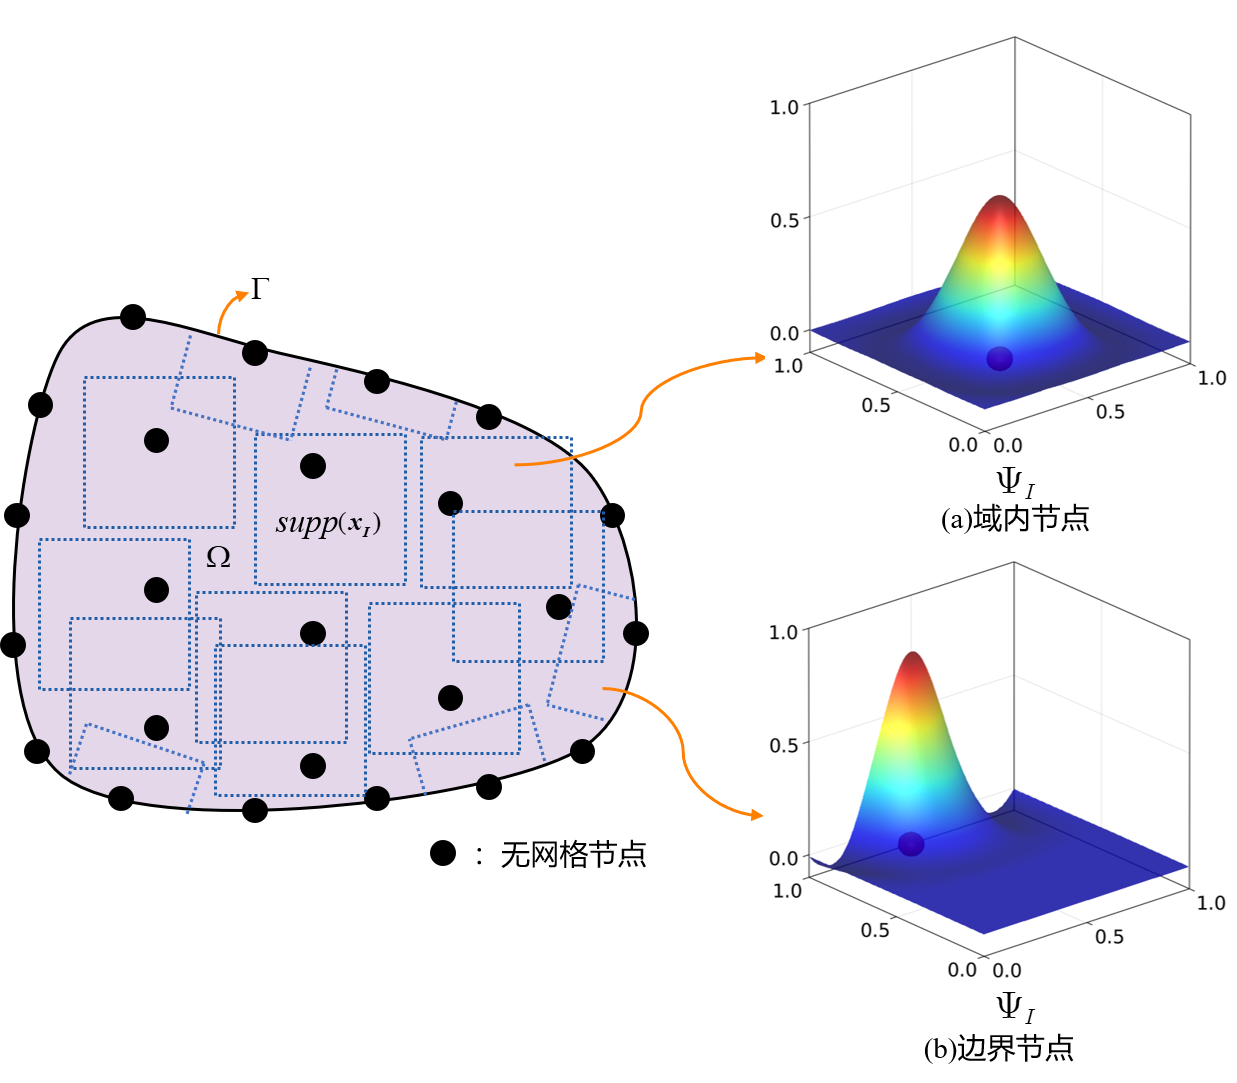
\includegraphics[scale=0.5]{figure/E/PSI.png}
    \caption{二维无网格离散示意图}\label{PSI}
\end{figure}\newpage
根据再生核近似理论[],无网格形函数可以假设为:
\begin{equation}\label{shapefunction}
\begin{split}
    \Psi_I(\pmb{x})=\sum_{I=1}^{N\!P}\pmb{p}^T(\pmb{x}_I-\pmb{x})\pmb{c}(\pmb{x})\phi_s(\pmb{x}_I-\pmb{x})
\end{split}
\end{equation}
式中,$\pmb{p}(\pmb{x})$表示为$p$阶的多项式基函数向量,表达式为:
\begin{equation}
\begin{split}
    \pmb{p}(\pmb{x})=\{1,x,y,\dotsb,x^iy^i,\dotsb,y^p\},0\le i+j \le p
\end{split}
\end{equation}
而$\phi_s(\pmb{x}_I-\pmb{x})$是附属于节点$\pmb{x}_I$的核函数,其影响域的大小由影响域尺寸$s$决定,核函数以及其影响域的大小共同决定了无网格形函数的局部紧支性和光滑性。对于二维问题,一般情况下核函数$\phi_s(\pmb{x}_I-\pmb{x})$的影响域为圆形域或者矩形域,可由下列公式得到:
\begin{equation}
\begin{split}
    \phi_s(\pmb{x}_I-\pmb{x})=\phi_{s_x}(r_x)\phi_{s_y}(r_y),r_x=\frac{\lvert x_I-x\rvert}{s_x},r_y=\frac{\lvert y_I-y \rvert}{s_y}
\end{split}
\end{equation}
其中$s_x$和$s_y$分别为$x$和$y$方向上影响域的大小,计算时一般使得两个方向上的影响域大小相等即$s_x=s_y=s$。选取核函数时一般遵循核函数阶次$m$大于等于基函数阶次$p(m\ge p)$的原则。针对二阶势问题的弹性力学问题,无网格基函数一般选择二阶或者三阶,而核函数$\phi_s(\pmb{x}_I-\pmb{x})$则选取三次样条函数:
\begin{equation}
\begin{split}
    \phi(r)=\frac{1}{3!}
\begin{cases}
    (2-2r)^3-4(1-2r)^3 &r\le \frac{1}{2}\\
    (2-2r)^3&\frac{1}{2}<r\le 1\\
    0&r>1
\end{cases}
\end{split}
\end{equation}\par
无网格形函数表达式(\ref{shapefunction})中的$\pmb{c}$为待定系数向量,该表达式可以通过满足再生条件确定:
\begin{equation}\label{regeneration conditions}
\begin{split}
    \sum_{I=1}^{N\!P}\Psi_I(\pmb{x})\pmb{p}(\pmb{x}_I-\pmb{x})=\pmb{0}
\end{split}
\end{equation}
将无网格形函数表达式(\ref{shapefunction})代入再生条件(\ref{regeneration conditions})中,可以得到:
\begin{equation}
\begin{split}
    \pmb{c}(\pmb{x})=\pmb{A}^{-1}(\pmb{x})\pmb{p}(\pmb{0})
\end{split}
\end{equation}
其中$\pmb{A}(\pmb{x})$表示矩量矩阵,表达式为:
\begin{equation}
\begin{split}
    \pmb{A}(\pmb{x})=\sum_{I=1}^{N\!P}\pmb{p}(\pmb{x}_I-\pmb{x})\pmb{p}^T(\pmb{x}_I-\pmb{x})\phi_s(\pmb{x}_I-\pmb{x})
\end{split}
\end{equation}\par
将$\pmb{c}(\pmb{x})$代入到式(\ref{shapefunction})中得到再生核无网格形函数的具体表达式为:
\begin{equation}\label{Pshapefunction}
\begin{split}
    \Psi_I(\pmb{x})=\pmb{p}^T(\pmb{0})\pmb{A}^{-1}(\pmb{x})\pmb{p}(\pmb{x}_I-\pmb{x})\phi_s(\pmb{x}_I-\pmb{x})
\end{split}
\end{equation}\par
无网格形函数$\Psi_I(\pmb{x})$的一阶和二阶导数分别为:
\begin{equation}
\begin{split}
    \Psi_{I,i}(x)=\left(\begin{matrix}
    \pmb p_{,i}^{T}(x_I-x)\pmb A^{-1}(x)\phi_s(x_I-x)\\
    +\pmb p^{T}(x_I-x)\pmb A_{,i}^{-1}\phi_s(x_I-x)\\
    \pmb p^{T}(x_I-x)\pmb A^{-1}(x)\phi _{s,i}(x_I-x)\\
    \end{matrix}\right)
    \pmb p(\pmb 0)
\end{split}
\end{equation}
\begin{equation}
\begin{split}
    \Psi_{I,ij}(x)=\left(\begin{matrix}
    \pmb p_{,ij}^{T}(x_I-x)\pmb A^{-1}(x)\phi_s(x_I-x)\\
    +\pmb p_{,i}^{T}(x_I-x)\pmb A_{,j}^{-1}(x)\phi_s(x_I-x)\\
    +\pmb p_{,i}^{T}(x_I-x)\pmb A^{-1}(x)\phi_{s,j}(x_I-x)\\
    +\pmb p^{T}(x_I-x)\pmb A_{,ij}^{-1}(x)\phi_s(x_I-x)\\
    +\pmb p_{,j}^{T}(x_I-x)\pmb A_{,i}^{-1}(x)\phi_s(x_I-x)\\
    +\pmb p^{T}(x_I-x)\pmb A_{,i}^{-1}(x)\phi_{s,j}(x_I-x)\\
    +\pmb p^{T}(x_I-x)\pmb A^{-1}(x)\phi_{s,ij}(x_I-x)\\
    +\pmb p_{,j}^{T}(x_I-x)\pmb A^{-1}(x)\phi_{s,i}(x_I-x)\\
    +\pmb p^{T}(x_I-x)\pmb A_{,j}^{-1}(x)\phi_{s,i}(x_I-x)\\
    \end{matrix}\right)
    \pmb p(\pmb 0)
\end{split}
\end{equation}
式中$\pmb A_{,i}^{-1}=-\pmb A^{-1}\pmb A_{,i}\pmb A^{-1},\pmb A_{,ij}^{-1}=-\pmb A^{-1}(\pmb A_{,ij}\pmb A^{-1}+\pmb A_{,i}\pmb A_{,j}^{-1}+\pmb A_{,j}\pmb A_{,i}^{-1})$,可以看出无网格形函数及其导数的计算都较为复杂。\par
图(\ref{DPASI})表示为二维情况下的无网格形函数导数图。根据图(\ref{PSI})、(\ref{DPASI})可以看出无网格形函数在全域上连续光滑,但在无网格节点处,形函数不具有插值性,因此无法像有限元法一样直接施加本质边界条件。
\begin{figure}[!h]
    \centering
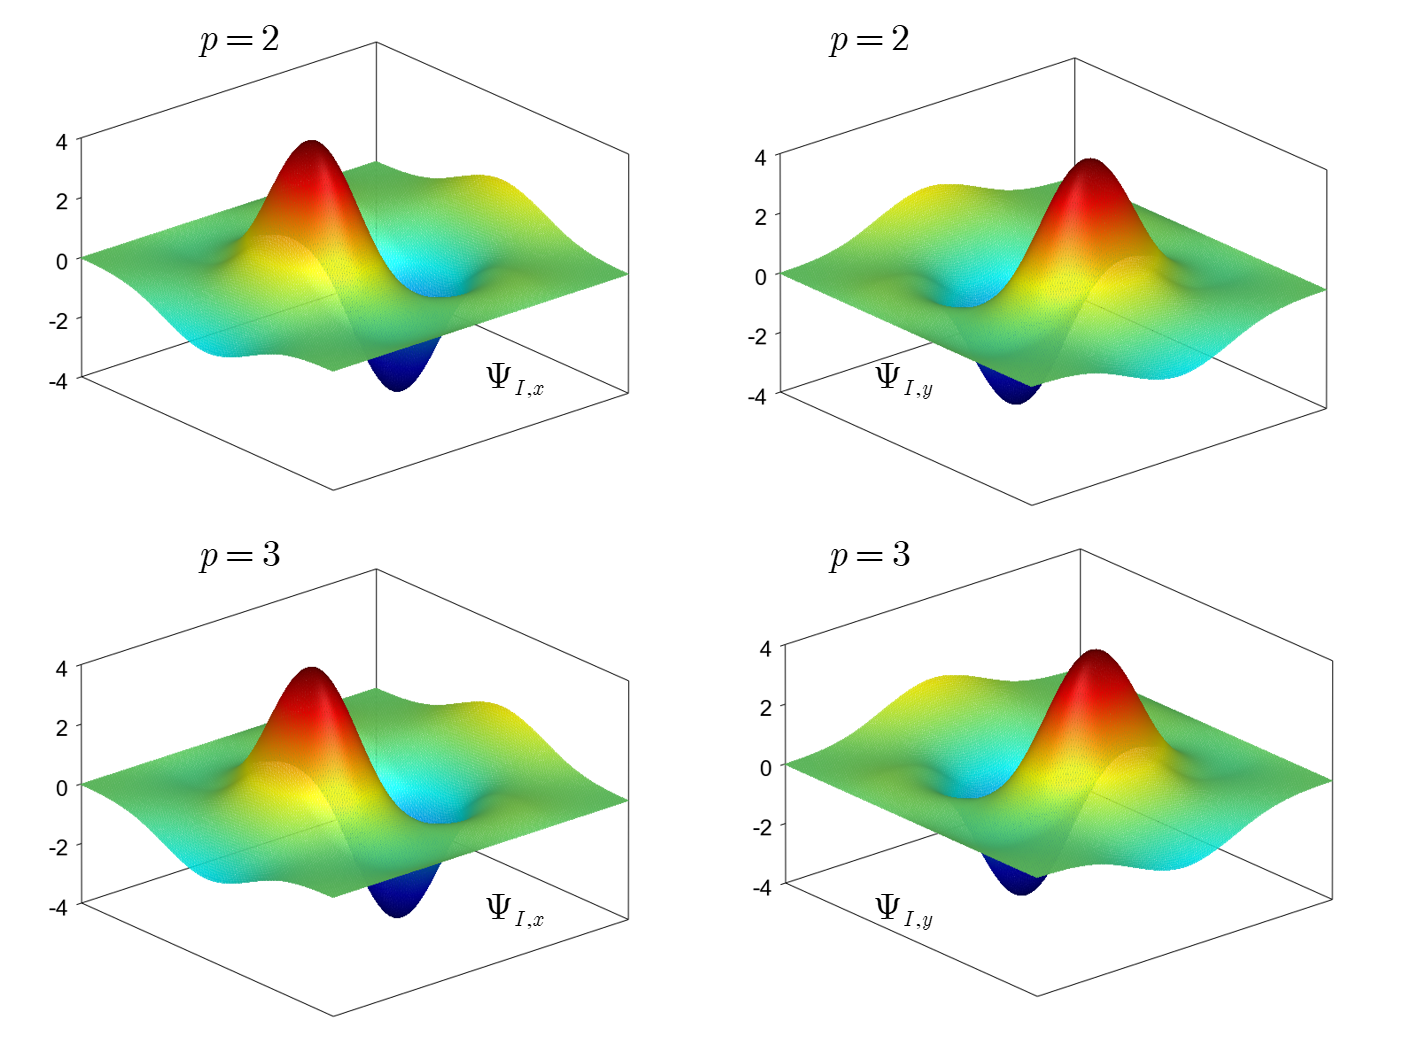
\includegraphics[scale=0.5]{figure/E/DPASI.png}
\caption{二维无网格形函数导数图}\label{DPASI}
\end{figure}\newpage
\subsection{应力离散与再生光滑梯度近似}
应力分量$\sigma_{ij}$采用在每个背景积分单元内建立局部的多项式进行离散。考虑如图(\ref{background})所示二维三角形背景积分单元,将求解域$\Omega$划分为一系列背景积分单元$\Omega_C$,$C=1,2,\dotsb,N\!C$,并且存在$\cup_{C=1}^{N\!C}\Omega_C\thickapprox\Omega$。
在背景积分单元$\Omega_C$内,假设应力分量$\sigma_{ij}$为任意的$p$阶多项式,则将离散后的应力分量$\sigma_{ij}$记为$\sigma^h_{ij}$:
其中,$\pmb{q}(\pmb{x})$为($p-1$)阶的单项式基向量,即$\pmb{q}(\pmb{x})=\pmb{p}^{[p-1]}(\pmb{x})$。$\pmb{a}_{ij}$为$\sigma_{ij}^h(\pmb{x})$在积分域$\Omega_C$内的常系数向量。\\
\begin{equation}\label{sigma}
\begin{split}
    \sigma^h_{ij}(\pmb{x})=\sum_{I=1}^{N\!P}\pmb{a}_{ij}^T\pmb{q}(\pmb{x}),\quad\text{in}\;\Omega_C
\end{split}
\end{equation}
\begin{figure}[!h]
    \centering
    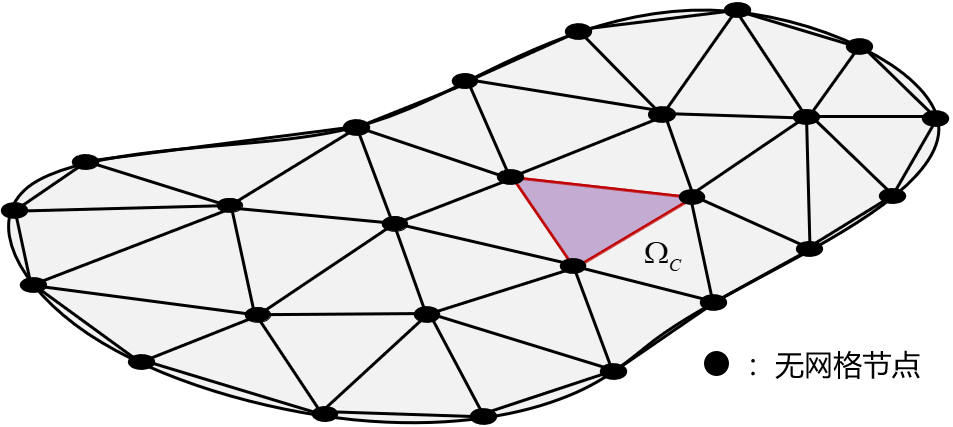
\includegraphics[scale=0.7]{figure/E/background.png}
    \caption{背景积分单元示意图}\label{background}
\end{figure}
此时,将(\ref{sigma})、(\ref{ui})代入(\ref{deltasigma})中可以得到:
\begin{equation}
\begin{split}
    \int_{\Omega_C}\delta\pmb{a}_{ij}\pmb{q}C^{-1}_{ijkl}\pmb{a}_{kl}\pmb{q}^Td\Omega&=\sum_{I=1}^{N\!P}\int_{\partial\Omega_C}\delta\pmb{a}_{ij}\pmb{q}n_j\Psi_I(\pmb{x})d\Gamma d_{iI}-\sum_{I=1}^{N\!P}\int_{\Omega_C}\delta\pmb{a}_{ij}\pmb{q}_{,j}\Psi_{I}(\pmb{x})d\Omega d_{iI}\\
     &-\sum_{I=1}^{N\!P}\int_{\Gamma^g\cap\partial\Omega_C}\delta\pmb{a}_{ij}\pmb{q}n_j\Psi_I(\pmb{x})d\Gamma d_{iI}+\int_{\Gamma^g\cap\partial\Omega_C}\delta\pmb{a}_{ij}\pmb{q}n_jg_id\Gamma
\end{split}
\end{equation}
等式两边同时消掉$\delta\pmb{a}_{ij}$,进一步得到:
\begin{equation}\label{a}
\begin{split}
        \int_{\Omega_C}\pmb{q}C^{-1}_{ijkl}\pmb{q}^Td\Omega\pmb{a}_{kl}&=\sum_{I=1}^{N\!P}\int_{\partial\Omega_C}\pmb{q}\Psi_I(\pmb{x})n_jd\Gamma d_{iI}-\sum_{I=1}^{N\!P}\int_{\Omega_C}\pmb{q}_{,j}\Psi_{I}(\pmb{x})d\Omega d_{iI}\\
         &-\sum_{I=1}^{N\!P}\int_{\Gamma^g\cap\partial\Omega_C}\pmb{q}\Psi_I(\pmb{x})n_jd\Gamma d_{iI}+\int_{\Gamma^g\cap\partial\Omega_C}\pmb{q}n_jg_id\Gamma
\end{split}
\end{equation}
对式(\ref{a})进行移项从而可以得到常系数向量$\pmb{a}_{ij}$的具体表达式为:
\begin{equation}\label{aij}
\begin{split}
 \pmb{a}_{ij}=C_{ijkl}\pmb{G}^{-1}(\sum_{I=1}^{N\!P}(\tilde{g}_{iI}-\bar{g}_{iI})d_{iI}+\hat{g}_{iI})
\end{split}
\end{equation}
其中:

\begin{align}
    \label{g1}&\pmb{G}=\int_{\Omega_C}\pmb{q}\pmb{q}^Td\Omega\\
    \label{g2} &\tilde{g}_{iI}=\int_{\partial\Omega_C}\pmb{q}\Psi_I(\pmb{x})n_jd\Gamma-\int_{\Omega_C}\pmb{q}_{,j}\Psi_{I}(\pmb{x})d\Omega\\
    \label{g3} &\bar{g}_{iI}=\int_{\Gamma^g\cap\partial\Omega_C}\pmb{q}\Psi_I(\pmb{x})n_jd\Gamma\\
   \label{g4} &\hat{g}_{iI}=\int_{\Gamma^g\cap\partial\Omega_C}\pmb{q}n_jg_id\Gamma
\end{align}

考虑经典的线弹性本构关系$\sigma_{ij}=C_{ijkl}\varepsilon_{kl},\varepsilon_{ij}=\frac{1}{2}(u_{i,j}+u_{j,i})$并将$\pmb{a}_{ij}$代入式(\ref{sigma})从而得到近似的应力分量$\sigma^h_{ij}(\pmb{x})$的具体表达式:
\begin{equation}\label{sigmah}
\begin{split}
    \sigma^h_{ij}(\pmb{x})=C_{ijkl}(\tilde{\varepsilon}^h_{kl}(\pmb{x})-\bar{\varepsilon}^h_{kl}(\pmb{x}))+C_{ijkl}\hat{\varepsilon}^h_{kl}(\pmb{x})
\end{split}
\end{equation}
其中:
\begin{equation}
\begin{split}
\begin{cases}\label{case1}
    \tilde{\varepsilon}^h_{ij}(\pmb{x})=\displaystyle\sum_{I=1}^{N\!P}\frac{1}{2}(\tilde{\Psi}_{I,i}(\pmb{x})d_{jI}+\tilde{\Psi}_{I,j}(\pmb{x})d_{iI})\\
    \tilde{\Psi}_{I,i}(\pmb{x})=\pmb{q}^T(\pmb{x})\pmb{G}^{-1}\tilde{g}_{iI}
\end{cases}
\end{split}
\end{equation}
\begin{equation}
\begin{split}
\begin{cases}\label{case2}
    \bar{\varepsilon}^h_{ij}(\pmb{x})=\displaystyle\sum_{I=1}^{N\!P}\frac{1}{2}(\bar{\Psi}_{I,i}(\pmb{x})d_{jI}+\bar{\Psi}_{I,j}(\pmb{x})d_{iI})\\
    \bar{\Psi}_{I,i}(\pmb{x})=\pmb{q}^T(\pmb{x})\pmb{G}^{-1}\bar{g}_{iI}
\end{cases}
\end{split}
\end{equation}
\begin{equation}
\begin{split}\label{case3}
    \hat{\varepsilon}_{ij}(\pmb{x})=\pmb{q}^T(\pmb{x})\pmb{G}^{-1}\hat{g}_{ij}
\end{split}
\end{equation}\par
此时,应力分量表达式中的$\tilde{\Psi}_{I,i}$为再生光滑梯度,根据再生光滑梯度理论[],再生光滑梯度可以通过直接构造得到,避免了传统无网格形函数梯度的复杂计算,提高了梯度计算效率。并且,再生光滑梯度
内嵌局部积分约束条件$\tilde{g}_{iI}$,可满足全域积分约束条件,从而保证算法的计算精度和误差收敛性。\par
为了方便起见,在实际计算分析中一般将张量表示转换为矩阵和向量表示,但两者完全等价。当考虑$xy$平面内的平面应力问题时,弹性本构关系为:
\begin{equation}
\begin{split}
    \left\{\begin{matrix}
    \sigma_{xx}\\\sigma_{yy}\\\sigma_{xy}
    \end{matrix}\right\}=\frac{E}{1-\nu^2}
    \left[\begin{matrix}
    1&\nu&0\\\nu&1&0\\0&0&\frac{1-\nu}{2}
    \end{matrix}\right]
    \left\{\begin{matrix}
    \varepsilon_{xx}\\\varepsilon_{yy}\\\gamma_{xy}
 \end{matrix}\right\}
\end{split}
\end{equation}
此时,近似应力分量$\pmb{\sigma}^h(\pmb{x})$式(\ref{sigmah})采用矩阵向量形式可以改写为:
\begin{equation}
\begin{split}
\pmb{\sigma}^h=\pmb{D}\sum_{I=1}^{N\!P}(\tilde{\pmb{B}}_I-\bar{\pmb{B}}_I)\pmb{d_I}+\pmb{D}\hat{\pmb{\varepsilon}}
\end{split}
\end{equation}
其中:
\begin{equation}
\begin{split}
    \pmb{\sigma}^h=\left\{\begin{matrix}
        \sigma_{xx}\\\sigma_{yy}\\\sigma_{xy}
        \end{matrix}\right\}\quad
    \pmb{D}=\frac{E}{1-\nu^2}
    \left[\begin{matrix}
    1&\nu&0\\\nu&1&0\\0&0&\frac{1-\nu}{2}
    \end{matrix}\right]\quad
    \hat{\pmb{\varepsilon}}=\left\{\begin{matrix}
        \varepsilon_{xx}\\\varepsilon_{yy}\\\gamma_{xy}
     \end{matrix}\right\}
\end{split}
\end{equation}
而$\pmb{d}_I=\{d_{1I},d_{2I}\}^T$为节点系数向量,$\tilde{\pmb{B}}_I\text{、}\bar{\pmb{B}}_I$分别是由再生光滑梯度$\tilde{\Psi}_{I,i}$和$\bar{\Psi}_{I,i}$组成的梯度矩阵,表达式分别为:
\begin{equation}
\begin{split}
    \tilde{\pmb{B}}_I(\pmb{x})= \left[\begin{matrix}\tilde{\Psi}_{I,x}(\pmb{x})&0\\0&\tilde{\Psi}_{I,y}(\pmb{x})\\\tilde{\Psi}_{I,y}(\pmb{x})&\tilde{\Psi}_{I,x}(\pmb{x}) \end{matrix}\right] 
\end{split}
\end{equation}
\begin{equation}
\begin{split}
    \bar{\pmb{B}}_I(\pmb{x})= \left[\begin{matrix}\bar{\Psi}_{I,x}(\pmb{x})&0\\0&\bar{\Psi}_{I,y}(\pmb{x})\\\bar{\Psi}_{I,y}(\pmb{x})&\bar{\Psi}_{I,x}(\pmb{x}) \end{matrix}\right] 
\end{split}
\end{equation}
\section{Hellinger-Reissner变分原理下的本质边界条件施加方法}
通过式(\ref{weak form1})看出基于Hellinger-Reissner变分原理得到的弱形式已经考虑了本质边界条件$\Gamma^g$和自然边界条件$\Gamma^t$。为了进一步了解关于采用Hellinger-Reissner变分原理在伽辽金无网格法中的本质边界条件。
此时将式(\ref{ui})、(\ref{sigma})代入弱形式(\ref{deltau})中可以得到:
\begin{equation}
\begin{split}
\sum_{C=1}^{N\!C}\sum_{I=1}^{N\!P}\delta d_{iI}(\int_{\partial\Omega_C}\Psi_I\pmb{q}^Tn_jd\Gamma&-\int_{\Omega_C}\Psi_I\pmb{q}_{,j}^Td\Omega-\int_{\Gamma^g\cap\partial\Omega_C}\Psi_I\pmb{q}^Tn_jd\Gamma)\pmb{a}_{ij}=\\
&\sum_{I=1}^{N\!P}\delta d_{iI}(\int_{\Gamma^t}\Psi_It_id\Gamma+\int_{\Omega}\Psi_Ib_id\Omega)
\end{split}
\end{equation}
引入式(\ref{g2})、(\ref{g3})将上式改写为:
\begin{equation}\label{1}
\begin{split}
    \sum_{C=1}^{N\!C}\sum_{I=1}^{N\!P}\delta d_{iI}(\tilde{g}_{jI}^T-\bar{g}_{jI}^T)\pmb{a}_{ij}=\sum_{I=1}^{N\!P}\delta\pmb{d}_I^T\pmb{f}_I=\delta\pmb{d}^T\pmb{f}
\end{split}
\end{equation}
其中$\delta\pmb{d}$为位移变分节点系数向量,$\pmb{f}$为外力向量,元素表达式为:
\begin{equation}
\begin{split}
    \pmb{f}_I=\int_{\Gamma^t}\Psi_I\pmb{t}d\Gamma+\int_{\Omega}\Psi_I\pmb{b}d\Omega
\end{split}
\end{equation}
式中$\pmb{t}=\{t_x,t_y\}^T\text{、}\pmb{b}=\{b_x,b_y\}^T$分别为外力向量和体力向量。进一步将式(\ref{aij})中的$\pmb{a}_{ij}$代入式(\ref{1})中从而得到:
\begin{equation}\label{inference}
\begin{split}
    \sum_{C=1}^{N\!C}\sum_{I=1}^{N\!P}\delta d_{iI}(\tilde{g}_{jI}^T-\bar{g}_{jI}^T)\pmb{a}_{ij}&=\sum_{C=1}^{N\!C}\sum_{I=1}^{N\!P}\delta d_{iI}(\tilde{g}_{jI}^T-\bar{g}_{jI}^T)C_{ijkl}\pmb{G}^{-1}(\sum_{J=1}^{N\!P}(\tilde{g}_{kJ}-\bar{g}_{kJ})d_{lJ}+\hat{g}_{kl})\\
    &=\sum_{C=1}^{N\!C}\sum_{I=1}^{N\!P}\sum_{J=1}^{N\!P}\delta d_{iI}\tilde{g}^T_{jI}C_{ijkl}\pmb{G}^{-1}\tilde{g}_{kJ}d_{lJ}\\
    &-\sum_{C=1}^{N\!C}\sum_{I=1}^{N\!P}\sum_{J=1}^{N\!P}\delta d_{iI}\tilde{g}^T_{jI}C_{ijkl}\pmb{G}^{-1}\bar{g}_{kJ}d_{lJ}\\
    &-\sum_{C=1}^{N\!C}\sum_{I=1}^{N\!P}\sum_{J=1}^{N\!P}\delta d_{iI}\bar{g}^T_{jI}C_{ijkl}\pmb{G}^{-1}\tilde{g}_{kJ}d_{lJ}\\
    &+\sum_{C=1}^{N\!C}\sum_{I=1}^{N\!P}\sum_{J=1}^{N\!P}\delta d_{iI}\bar{g}^T_{jI}C_{ijkl}\pmb{G}^{-1}\bar{g}_{kJ}d_{lJ}\\
    &-\sum_{C=1}^{N\!C}\sum_{I=1}^{N\!P}\delta d_{iI}\tilde{g}_{jI}^TC_{ijkl}\pmb{G}^{-1}\hat{g}_{kl}\\
    &+\sum_{C=1}^{N\!C}\sum_{I=1}^{N\!P}\delta d_{iI}\bar{g}_{jI}^TC_{ijkl}\pmb{G}^{-1}\hat{g}_{kl}
\end{split}
\end{equation}
通过引入式(\ref{g1})、(\ref{case1})对式(\ref{inference})中的第一项进行推导可得:
\begin{equation}
\begin{split}
    \sum_{C=1}^{N\!C}\sum_{I=1}^{N\!P}\sum_{J=1}^{N\!P}\delta d_{iI}\tilde{g}^T_{jI}C_{ijkl}\pmb{G}^{-1}\tilde{g}_{kJ}d_{lJ}&=\sum_{C=1}^{N\!C}\sum_{I=1}^{N\!P}\sum_{J=1}^{N\!P}\delta d_{iI}\tilde{g}^T_{jI}C_{ijkl}\pmb{G}^{-1}\pmb{G}\pmb{G}^{-1}\tilde{g}_{kJ}d_{lJ}\\
&=\sum_{C=1}^{N\!C}\sum_{I=1}^{N\!P}\sum_{J=1}^{N\!P}\delta d_{iI}\int_{\Omega_C}\tilde{g}_{jI}^T\pmb{G}^{-1}\pmb{q}(\pmb{x})C_{ijkl}\pmb{q}^T(\pmb{x})\pmb{G}^{-1}\tilde{g}_{kJ}d\Omega d_{lJ}\\
&=\sum_{C=1}^{N\!C}\int_{\Omega_C}\sum_{I=1}^{N\!P}\tilde{\Psi}_{I,j}\delta d_{iI}C_{ijkl}\sum_{J=1}^{N\!P}\tilde{\Psi}_{I,k}d_{lJ}d\Omega\\
&=\sum_{C=1}^{N\!C}\int_{\Omega_C}\delta\tilde{\varepsilon}_{ij}^hC_{ijkl}\tilde{\varepsilon}_{kl}^hd\Omega\\
&=\sum_{I=1}^{N\!P}\sum_{J=1}^{N\!P}\delta\pmb{d}^T_I\int_{\Omega}\tilde{\pmb{B}}_I^T\pmb{D}\tilde{\pmb{B}}_Jd\Omega\pmb{d}_J\\
&=\delta\pmb{d}^T\pmb{K}\pmb{d}
\end{split}
\end{equation}
通过引入式(\ref{g3})、(\ref{case1})、(\ref{ui})对式(\ref{inference})中的第二、三项进行推导可得:
\begin{equation}
\begin{split}
    &-\sum_{C=1}^{N\!C}\sum_{I=1}^{N\!P}\sum_{J=1}^{N\!P}\delta d_{iI}C_{ijkl}(\bar{g}_{jI}^T\pmb{G}^{-1}\tilde{g}_{kJ}+\tilde{g}_{jI}^T\pmb{G}^{-1}\bar{g}_{kJ})d_{lJ}\\
    &=-\sum_{C=1}^{N\!C}\sum_{I=1}^{N\!P}\sum_{J=1}^{N\!P}\delta d_{iI}(\int_{\Gamma^g\cap\partial\Omega_C}\Psi_In_jC_{ijkl}\pmb{q}\pmb{G}^{-1}\tilde{g}_{kJ}d\Gamma+\int_{\Gamma^g\cap\partial\Omega_C}C_{ijkl}\pmb{q}\pmb{G}^{-1}\tilde{g}_{jI}n_k\Psi_Jd\Gamma)d_{lJ}\\
    &=-\sum_{C=1}^{N\!C}(\int_{\Gamma^g\cap\partial\Omega_C}\sum_{I=1}^{N\!P}\Psi_I\delta d_{iI}n_jC_{ijkl}\sum_{J=1}^{N\!P}\tilde{\Psi}_{J,k}d_{lJ}d\Gamma+\int_{\Gamma^g\cap\partial\Omega_C}C_{ijkl}\sum_{J=1}^{N\!P}\tilde{\Psi}_{I,j}\delta d_{iI}n_k\sum_{I=1}^{N\!P}\Psi_Jd_{lJ}d\Gamma)\\
    &=-\sum_{C=1}^{N\!C}(\int_{\Gamma^g\cap\partial\Omega}\delta u_i^hn_jC_{ijkl}\tilde{\varepsilon}_{kl}^hd\Gamma+\int_{\Gamma^g\cap\partial\Omega_C}\delta\tilde{\varepsilon}_{ij}^hC_{ijkl}n_ku^h_ld\Gamma)\\
    &=-\sum_{I=1}^{N\!P}\sum_{J=1}^{N\!P}\delta\pmb{d}_I^T(\int_{\Gamma^g}\Psi_I\pmb{N}\pmb{D}\tilde{\pmb{B}}_Jd\Gamma+\int_{\Gamma^g}\tilde{\pmb{B}}_I^T\pmb{D}\pmb{N}^T\Psi_Jd\Gamma)\pmb d_J\\
    &=\delta\pmb{d}^T\tilde{\pmb{K}}\pmb{d}
\end{split}
\end{equation}
其中$\pmb{N}$为法向量矩阵:
\begin{equation}
\begin{split}
    \pmb{N}=\left[\begin{matrix}n_x&0&n_y\\0&n_y&n_x
    \end{matrix}\right] 
\end{split}
\end{equation}
通过引入式(\ref{g3})、(\ref{case2})对式(\ref{inference})中的第四项进行推导可得:
\begin{equation}
\begin{split}
    \sum_{C=1}^{N\!C}\sum_{I=1}^{N\!P}\sum_{J=1}^{N\!P}\delta d_{iI}C_{ijkl}\bar{g}^T_{jI}\pmb{G}^{-1}\bar{g}_{kJ}d_{lJ}
    &=\sum_{C=1}^{N\!C}\sum_{I=1}^{N\!P}\sum_{J=1}^{N\!P}\delta d_{iI}\int_{\Gamma^g\cap\partial\Omega_C}C_{ijkl}\bar{g}_{jI}^T\pmb{G}^{-1}\pmb{q}\Psi_Jn_kd\Gamma d_{lJ}\\
    &=\sum_{C=1}^{N\!C}\int_{\Gamma^g\cap\partial\Omega_C}C_{ijkl}\sum_{J=1}^{N\!P}\bar{\Psi}_{I,j}\delta d_{iI}n_k\sum_{J=1}^{N\!P}\Psi_{J}d_{lJ}d\Gamma\\
    &=\sum_{C=1}^{N\!C}\int_{\Gamma^g\cap\partial\Omega_C}C_{ijkl}\delta\bar{\varepsilon}_{ij}^hn_ku_ld\Gamma\\
    &=\sum_{I=1}^{N\!P}\sum_{J=1}^{N\!P}\delta\pmb{d}_I^T\int_{\Gamma^g\cap\partial\Omega_C}\bar{\pmb{B}}_I^T\pmb{D}\pmb{N}^T\Psi_Jd\Gamma\pmb{d}_J\\
    &=\delta\pmb{d}^T\bar{\pmb{K}}\pmb{d}
\end{split}
\end{equation}
通过引入式(\ref{g4})、(\ref{case1})对式(\ref{inference})中的第五项进行推导可得:
\begin{equation}
\begin{split}
    -\sum_{C=1}^{N\!C}\sum_{I=1}^{N\!P}\delta d_{iI}C_{ijkl}\tilde{g}^T_{jI}\pmb{G}^{-1}\hat{g}_{kl}
    &=-\sum_{C=1}^{N\!C}\sum_{I=1}^{N\!P}\delta d_{iI}C_{ijkl}\tilde{g}^T_{jI}\pmb{G}^{-1}\int_{\Gamma^g\cap\partial\Omega_C}\pmb{q}n_lg_kd\Gamma\\
    &=-\sum_{C=1}^{N\!C}\int_{\Gamma^g\cap\partial\Omega_C}C_{ijkl}\sum_{I=1}^{N\!P}\tilde{\Psi}_{I,j}\delta d_{iI}n_lg_kd\Gamma\\
    &=-\sum_{C=1}^{N\!C}\int_{\Gamma^g\cap\partial\Omega_C}C_{ijkl}\delta\tilde{\varepsilon}_{ij}^hn_lg_kd\Gamma\\
    &=-\sum_{I=1}^{N\!P}\delta\pmb{d}_I^T\int_{\Gamma^g\cap\partial\Omega_C}\tilde{\pmb{B}}_I^T\pmb{D}\pmb{N}^T\pmb{g}d\Gamma\\
    &=\delta\pmb{d}^T\tilde{\pmb{f}}
\end{split}
\end{equation}
通过引入式(\ref{g4})、(\ref{case2})对式(\ref{inference})中的第六项进行推导可得:
\begin{equation}
\begin{split}
    \sum_{C=1}^{N\!C}\sum_{I=1}^{N\!P}\delta d_{iI}C_{ijkl}\bar{g}^T_{jI}\pmb{G}^{-1}\hat{g}_{kl}
    &=\sum_{C=1}^{N\!C}\sum_{I=1}^{N\!P}\delta d_{iI}C_{ijkl}\bar{g}^T_{jI}\pmb{G}^{-1}\int_{\Gamma^g\cap\partial\Omega_C}\pmb{q}n_lg_kd\Gamma\\
    &=\sum_{C=1}^{N\!C}\int_{\Gamma^g\cap\partial\Omega_C}C_{ijkl}\sum_{I=1}^{N\!P}\bar{\Psi}_{I,j}\delta d_{iI}n_lg_kd\Gamma\\
    &=\sum_{C=1}^{N\!C}\int_{\Gamma^g\cap\partial\Omega_C}C_{ijkl}\delta\bar{\varepsilon}_{ij}^hn_lg_kd\Gamma\\
    &=\sum_{I=1}^{N\!P}\delta\pmb{d}_I^T\int_{\Gamma^g\cap\partial\Omega_C}\bar{\pmb{B}}_I^T\pmb{D}\pmb{N}^T\pmb{g}d\Gamma\\
    &=\delta\pmb{d}^T\bar{\pmb{f}}
\end{split}
\end{equation}
此时,式(\ref{inference})通过化简可以得到:
\begin{equation}\label{simplify}
\begin{split}
    \sum_{C=1}^{N\!C}\sum_{I=1}^{N\!P}\delta d_{iI}(\tilde{g}_{jI}^T-\bar{g}_{jI}^T)\pmb{a}_{ij}=
    \delta\pmb{d}^T(\pmb{K}+\tilde{\pmb{K}}+\bar{\pmb{K}})\pmb{d}-\delta\pmb{d}^T(\tilde{\pmb{f}}+\bar{\pmb{f}})
\end{split}
\end{equation}
将式(\ref{simplify})代入到式(\ref{1})中从而得到离散的平衡方程:
\begin{equation}\label{equationE}
\begin{split}
    \delta\pmb{d}^T(\pmb{K}+&\tilde{\pmb{K}}+\bar{\pmb{K}})\pmb{d}-\delta\pmb{d}^T(\tilde{\pmb{f}}+\bar{\pmb{f}})=\delta\pmb{d}^T\pmb{f}\\
    &(\pmb{K}+\pmb{\tilde{K}}+\pmb{\bar{K}})\pmb{d}=\pmb{f}+\tilde{\pmb{f}}+\bar{\pmb{f}}
\end{split}
\end{equation}\par
为了保证离散弱形式的变分一致性在求解式(\ref{equationE})的过程中,引入的数值积分在求解的各个过程也需要保持一致。如图(\ref{strain})所示,基于Hellinger-Reissner变分原理下的本质边界条件施加方法的
本质边界条件施加方法需要两套数值积分点,$\tilde{g}$和$\bar{g}$中的数值积分方案需要与$\tilde{\pmb{K}}$,$\bar{\pmb{K}}$,$\pmb{f}$,$\tilde{\pmb{f}}$和$\bar{\pmb{f}}$保持一致。\par
\begin{figure}[!h]
    \centering
    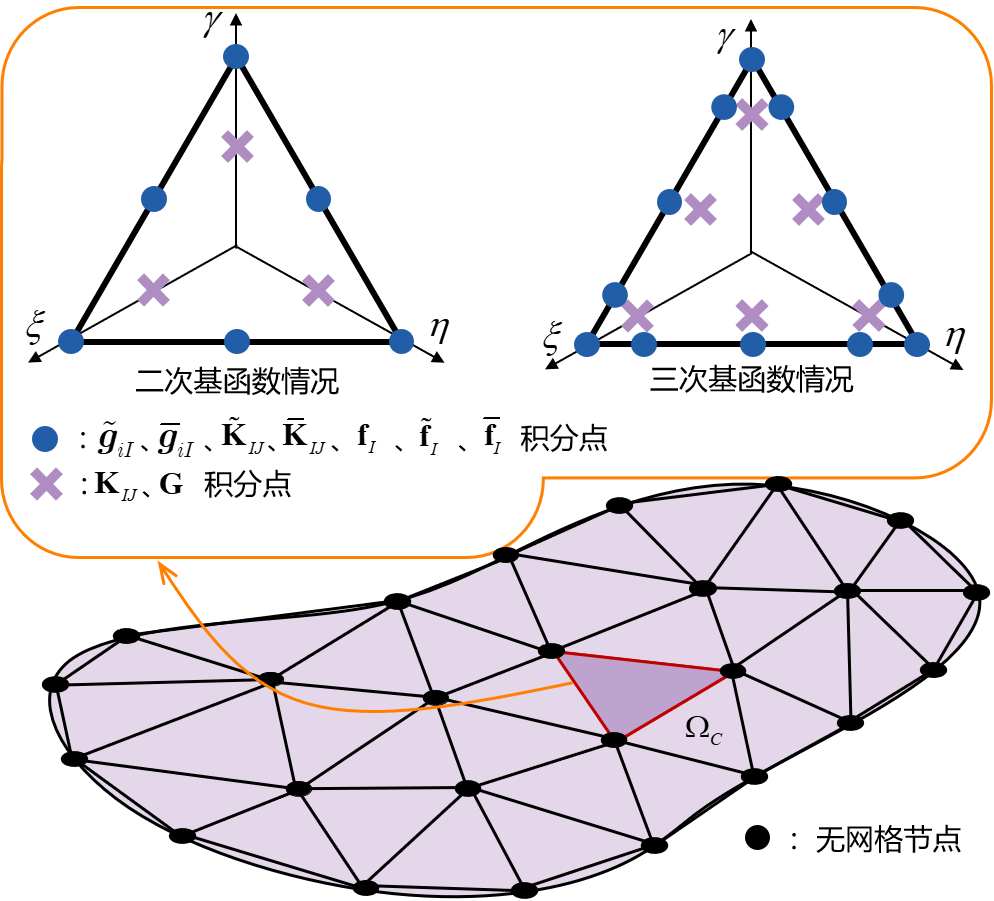
\includegraphics[scale=0.5]{figure/E/strain.png}
    \caption{优化的数值积分方案}\label{strain}
\end{figure}\newpage
同时,基于Hellinger-Reissner变分原理的本质边界条件施加方法中的再生光滑梯度构造过程中需要计算积分点处无网格形函数。采用无网格再生光滑梯度积分法,减小形函数的计算量、提高计算效率。
利用积分点在背景积分单元间的共享特性,从全域上优化整体求解过程中积分点的数量,提高计算效率,具体数值积分方案如下表:\par    
\begin{table}[h]
\caption{\textbf{二次基函数无网格法优化的数值积分方案}}
\centering
\begin{tabular}{cccccc}
   \toprule
   数值积分点&$\xi$ & $\eta$ & $\gamma$ & $w$ & $w_B$\\
   \midrule
   \begin{minipage}[b]{0.3\columnwidth}
    \centering
    \raisebox{-.5\height}{
\includegraphics{figure/E/point.png}}
\end{minipage}&
   $\frac{2}{3}$ & $\frac{1}{6}$& $\frac{1}{6}$ & $\frac{1}{3}$\\
   \midrule
      \begin{minipage}[b]{0.3\columnwidth}
    \centering
    \raisebox{-.5\height}{
\includegraphics{figure/E/point2.png}}
\end{minipage}&
   $\frac{1}{2}$ & $\frac{1}{2}$ &0 & $\frac{1}{6}$\\
   &1&0&0&$\frac{2}{3}$&$\frac{1}{3}$\\
   \bottomrule
\end{tabular}
\end{table}
\begin{table}[h]
    \caption{\textbf{三次基函数无网格法优化的数值积分方案}}
    \centering
    \begin{tabular}{cccccc}
   \toprule
   数值积分点&$\xi$ & $\eta$ & $\gamma$ & $w$ & $w_B$\\
   \midrule
\begin{minipage}[b]{0.3\columnwidth}
    \centering
    \raisebox{-.5\height}{
\includegraphics{figure/E/point.png}}
\end{minipage}&
$\eta_a$&$\frac{1-\xi_a}{2}$&$\frac{1-\xi_a}{2}$&$w_a$\\
&$\eta_b$&$\eta_b$&$\frac{1-\xi_b}{2}$&$w_b$\\
$\xi_a=0.10810301816870,w_a=0.223381589678011$\\
$\xi_b=0.816847572980459,w_b=0.109951743655322$\\
\midrule
\begin{minipage}[b]{0.3\columnwidth}
    \centering
    \raisebox{-.5\height}{
\includegraphics{figure/E/point2.png}}
\end{minipage}&
$\frac{1}{3}$&$\frac{1}{3}$&$\frac{1}{3}$&$\frac{9}{20}$\\
&$1$&$0$&$0$&$-\frac{1}{30}$&$\frac{1}{20}$\\
&$\frac{1}{2}$&$\frac{1}{2}$&$0$&$\frac{4}{135}$&$\frac{16}{46}$\\
&$\frac{7+\sqrt{21}}{14}$&$\frac{7+\sqrt{21}}{14}$&$0$&$\frac{49}{540}$&$\frac{49}{180}$\\
\bottomrule
\end{tabular}
\end{table}
\section{数值算例}
\subsection{分片实验}
首先采用线性、二次和三次弹性力学分片实验验证采用传统高斯积分法和再生光滑梯度积分法的不同本质边界条件施加方法下是否满足积分约束条件的情况。
分片实验考虑求解域为边长等于1的正方形,求解域的四边施加本质边界条件。其分片实验的精确解如下:
\begin{equation}
\begin{split}
    \begin{cases}
        u_x(x,y)=(1+2x+3y)^n\\
        u_y(x,y)=(4+5x+6y)^n
    \end{cases}
\end{split}
\end{equation}
其中,$n=1,2,3$表示线性、二次和三次分片实验。如图(\ref{patchtestmeshfree})所示,分片实验采用$11\times 11$的非均匀节点离散求解域。针对二次基函数的无网格近似,采用线性和二次分片实验进行测试,核函数相对影响域在二次基函数情况下为2.5;
三次基函数的无网格近似采用二次和三次分片实验进行测试,核函数相对影响域在三次基函数情况下为3.5。\par
\begin{figure}[!h]
    \centering
    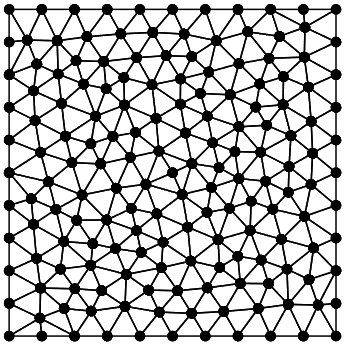
\includegraphics[scale=0.7]{figure/E/patchtestmeshfree.png}
    \caption{分片实验无网格离散模型}\label{patchtestmeshfree}
\end{figure}
分别采用位移误差$L_2$-Error和能量误差$H_1$-Error详细对比所提方法的计算精度
\begin{equation}
\begin{split}
    L_2\text{-Error}=\sqrt{\int_{\Omega}(u_i-u_i^h)(u_i-u_i^h)d\Omega}
\end{split}
\end{equation}
\begin{equation}
    \begin{split}
        H_1\text{-Error}=\sqrt{\frac{1}{2}\int_{\Omega}(\sigma_{ij}-\sigma_{ij}^h)C_{ijkl}^{-1}(\sigma_{ij}-\sigma_{ij}^h)d\Omega}
    \end{split}
    \end{equation}\par
在数值结果中,“GI”表示采用的是传统高斯积分法,“RKGSI”表示采用的是再生光滑梯度积分法。“Penalty”、“LM”和“Nitsche”分别表示罚函数法、拉格朗日乘子法和Nitsche法三种常见的本质边界条件施加方法。“RKGSI-HR”则表示的是本章提出的
基于Hellinger-Reissner变分原理的本质边界条件施加方法。在以下的数值求解过程中,为了保证拉格朗日乘子法的稳定性,拉格朗日乘子统一采用线性有限元形函数进行离散。针对二次基函数的求解,高斯积分法“GI”的求解域$\Omega$的积分采用13点高斯积分,边界$\Gamma$积分采用3点高斯积分
;针对三次基函数的求解,高斯积分法“GI”的求解域$\Omega$的积分采用16点高斯积分,边界$\Gamma$积分采用5点高斯积分。二次和三次基函数的无网格法分片试验结果如下:\par
\begin{table}[h]
    \caption{\textbf{二次基函数无网格法分片实验结果}}
    \centering
   \begin{tabular}{ccccc}
   \toprule
   &$\quad$ &线性分片实验 &$\quad$ &二次分片实验\\
   \midrule
   &$L_2$-Error$\quad$&$H_1$-Error&$L_2$-Error$\quad$&$H_1$-Error\\
   \midrule
   GI-Penalty&$7.7\times10^{-6}$&$2.7\times10^{-4}$&$1.2\times10^{-5}$&$2.6\times10^{-4}$\\
   GI-LM&$1.0\times10^{-4}$&$4.7\times10^{-3}$&$1.5\times10^{-4}$&$4.3\times10^{-3}$\\
   GI-Nitsche&$8.1\times10^{-6}$&$2.8\times10^{-4}$&$1.3\times10^{-5}$&$2.8\times10^{-4}$\\
  RKGSI-Penalty&$7.9\times10^{-8}$&$2.0\times10^{-6}$&$1.4\times10^{-7}$&$2.1\times10^{-6}$\\
  RKGSI-LM&$8.6\times10^{-5}$&$4.0\times10^{-3}$&$1.4\times10^{-4}$&$3.7\times10^{-3}$\\
  RKGSI-Nitsche&$2.1\times10^{-15}$&$4.0\times10^{-14}$&$2.2\times10^{-15}$&$2.7\times10^{-14}$\\
  RKGSI-HR&$2.0\times10^{-15}$&$3.2\times10^{-14}$&$2.2\times10^{-15}$&$2.1\times10^{-14}$\\
   \bottomrule
   \end{tabular}
   \end{table}
   \begin{table}[h]
    \caption{\textbf{三次基函数无网格法分片实验结果}}
    \centering
   \begin{tabular}{ccccc}
   \toprule
   &$\quad$ &二次分片实验 &$\quad$ &三次分片实验\\
   \midrule
   &$L_2$-Error$\quad$&$H_1$-Error&$L_2$-Error$\quad$&$H_1$-Error\\
   \midrule
   GI-Penalty&$9.1\times10^{-6}$&$2.1\times10^{-4}$&$1.2\times10^{-5}$&$2.0\times10^{-4}$\\
   GI-LM&$2.9\times10^{-4}$&$9.3\times10^{-3}$&$4.0\times10^{-4}$&$9.3\times10^{-3}$\\
   GI-Nitsche&$1.1\times10^{-5}$&$2.8\times10^{-4}$&$1.4\times10^{-5}$&$2.7\times10^{-4}$\\
  RKGSI-Penalty&$1.4\times10^{-7}$&$2.1\times10^{-6}$&$2.0\times10^{-7}$&$2.7\times10^{-6}$\\
  RKGSI-LM&$3.0\times10^{-4}$&$9.8\times10^{-3}$&$4.2\times10^{-4}$&$9.8\times10^{-3}$\\
  RKGSI-Nitsche&$3.6\times10^{-15}$&$1.0\times10^{-13}$&$4.6\times10^{-15}$&$9.5\times10^{-14}$\\
  RKGSI-HR&$3.1\times10^{-15}$&$1.0\times10^{-13}$&$3.5\times10^{-15}$&$7.4\times10^{-14}$\\
   \bottomrule
   \end{tabular}
   \end{table}\newpage
表3.3和表3.4分别为具有二次、三次基函数无网格法的分片试验结果,
从表中可以看出,由于传统高斯积分法不满足积分约束条件,所以即使采用高阶高斯积分的罚函数法(GI-Penalty)、拉格朗日乘子法(GI-LM)和Nitsche法(GI-Nitsche)均不能通过分片试验。
当采用满足积分约束条件的再生光滑梯度积分法时,此时由于罚函数法(RKGSI-Penalty)不具有变分一致性,也无法通过分片试验;
拉格朗日乘子法(RKGSI-LM)由于其拉格朗日乘子采用线性形函数进行离散,无法与再生光滑梯度相匹配,也无法通过分片试验;
当采用Nitsche法(RKGSI-Nitsche)和基于Hellinger-Reissner变分原理(RKGSI-HR)的本质边界条件施加方法时,均可以通过分片试验,即满足积分约束条件。
\subsection{悬臂梁问题}
首先考虑经典弹性力学二维悬臂梁问题,如图(\ref{cantilever})所示,悬臂梁的长和宽分别为$L=48$,$D=12$,同时悬臂梁的左端为固定支座,
右端沿着$y$轴正方向施加外部荷载$P=1000$。悬臂梁的材料系数为杨氏模量$E=3\times10^6$、泊松比$\nu=0.3$。
根据圣维南原理和平面应力假设,悬臂梁问题的解析解为:
\begin{equation}
\begin{split}
\begin{cases}
    u = -\frac{Py}{6EI}[(6L-3x)x + (2+\nu)(y^2 - \frac{D^2}{4})] \\
    v = \frac{P}{6EI}[3\nu y^2(L-x) + (4+5\nu)\frac{D^2x}{4} + (3L-x)x^2]
\end{cases}
\end{split}
\end{equation}\par
与之相对应的应力分量为:
\begin{equation}
\begin{split}
\begin{cases}
   \sigma_{xx}=-\frac{P(L-x)y}{I}\\
   \sigma_{yy}=0\\
   \sigma_{xy}=\frac{P}{2I}(\frac{D^2}{4}-y^2)
\end{cases}
\end{split}
\end{equation}
\begin{figure}[H]
    \centering
    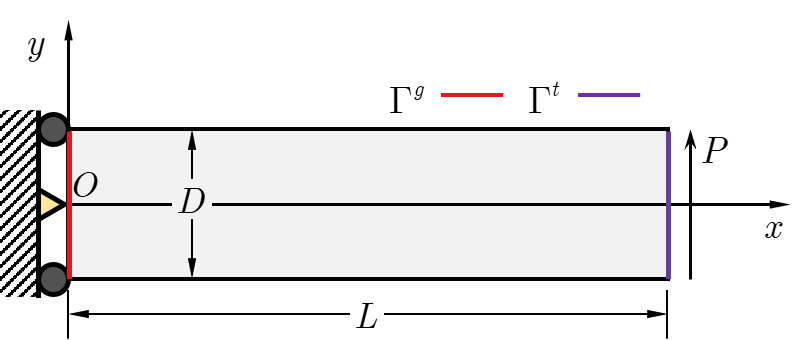
\includegraphics[scale=0.7]{figure/E/cantilever/cantilever.png}
    \caption{悬臂梁问题模型}\label{cantilever}
\end{figure}
如图(\ref{cantilever})所示,悬臂梁的左端施加自然边界条件$\Gamma^t$,右端施加强制边界条件$\Gamma^g$。
悬臂梁求解域分别通过图(\ref{cantilever.mesh})所示采用$\text{(a)}5\times7$、$\text{(b)}9\times33$、$\text{(c)}17\times65$、$\text{(d)}33\times129$的
四个疏密不同的节点进行离散。对于采用二次基函数的悬臂梁算例问题,传统高斯积分法采用13点高斯积分,核函数的相对影响域为2.5。
\begin{figure}[H]
    \centering
    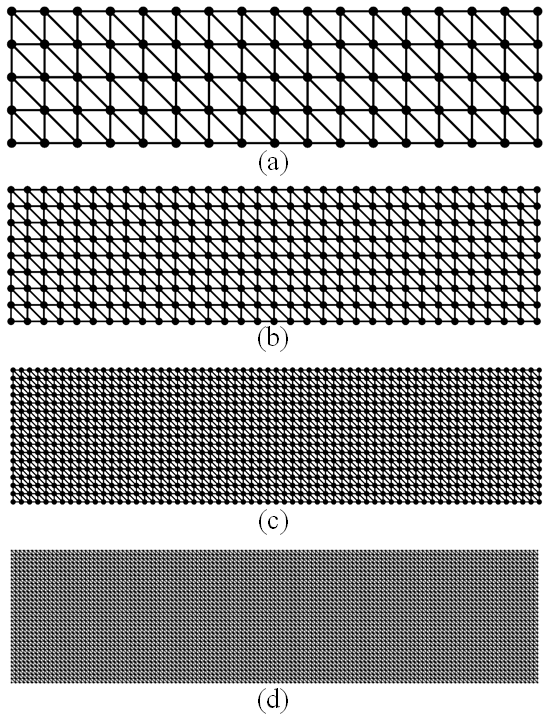
\includegraphics[scale=0.7]{figure/E/cantilever/cantilever.mesh.png}
    \caption{悬臂梁问题节点模型}\label{cantilever.mesh}
\end{figure}
图(\ref{CL2})、(\ref{CH1})为悬臂梁问题的位移误差和能量误差对比图。从图中可以看出采用再生光滑梯度积分法(RKGSI)的本质边界条件施加方法的计算精度优于采用高斯积分法(GI)的本质条件施加方法,
并且由于传统高斯积分法和采用再生光滑梯度积分法的罚函数法(RKGSI-Penalty)和拉格朗日乘子法(RKGSI-LM)不具有变分一致性,无法达到理论误差收敛率,而基于Hellinger-Reissner变分原理下的本质边界条件施加方法(RKGSI-HR)和Nitshce法(RKGSI-Nitsche)均可达到理论误差收敛率,但相较于RKGSI-Nitsche法,所提出的RKGSI-HR法无需引入人工参数。\par
图(\ref{CCPUTime})为悬臂梁问题的节点数和计算时间的效率对比图。从整体来看采用再生光滑梯度积分法(RKGSI)的计算效率明显高于传统高斯积分法(GI)。
图(\ref{Ccaculate})为悬臂梁问题的本质边界条件施加效率分析图。该图为施加强制边界$\Gamma^g$过程中计算形函数及梯度和组装相对应的刚度矩阵和力向量所用时间对比图。
从图中可以看出,罚函数法和拉格朗日乘子法在计算形函数及其梯度所用的时间相同且所用时间最少,这是由于罚函数法和拉格朗日乘子法在计算过程中只需要计算无网格形函数本身,无需计算无网格形函数梯度,
而Nitsche法和HR法也无需计算无网格形函数梯度,但需要计算再生光滑梯度,Nitshce法这部分所用的时间是罚函数法和拉格朗日乘子法的5.6倍,而HR法是1.6倍,HR法的计算效率高于Nitsche法。
组装相应的刚度矩阵和力向量这部分所用的时间上,Nitshe法和HR法计算效率基本相同。
从整体上来看,拉格朗日乘子法和罚函数法的效率优于HR法和Nitsche法,但拉格朗日乘子法和罚函数法不具有变分一致性无法达到理论误差收敛率。
因此,总体来说,相较于传统的本质边界条件施加方法,基于Hellinger-Reissner变分原理的本质边界条件施加方法(RKGSI-HR)能够达到理论误差收敛率,有效提高计算精度,相较于Nitsche法而言计算效率也更高。
\begin{figure}[H]
    \centering
    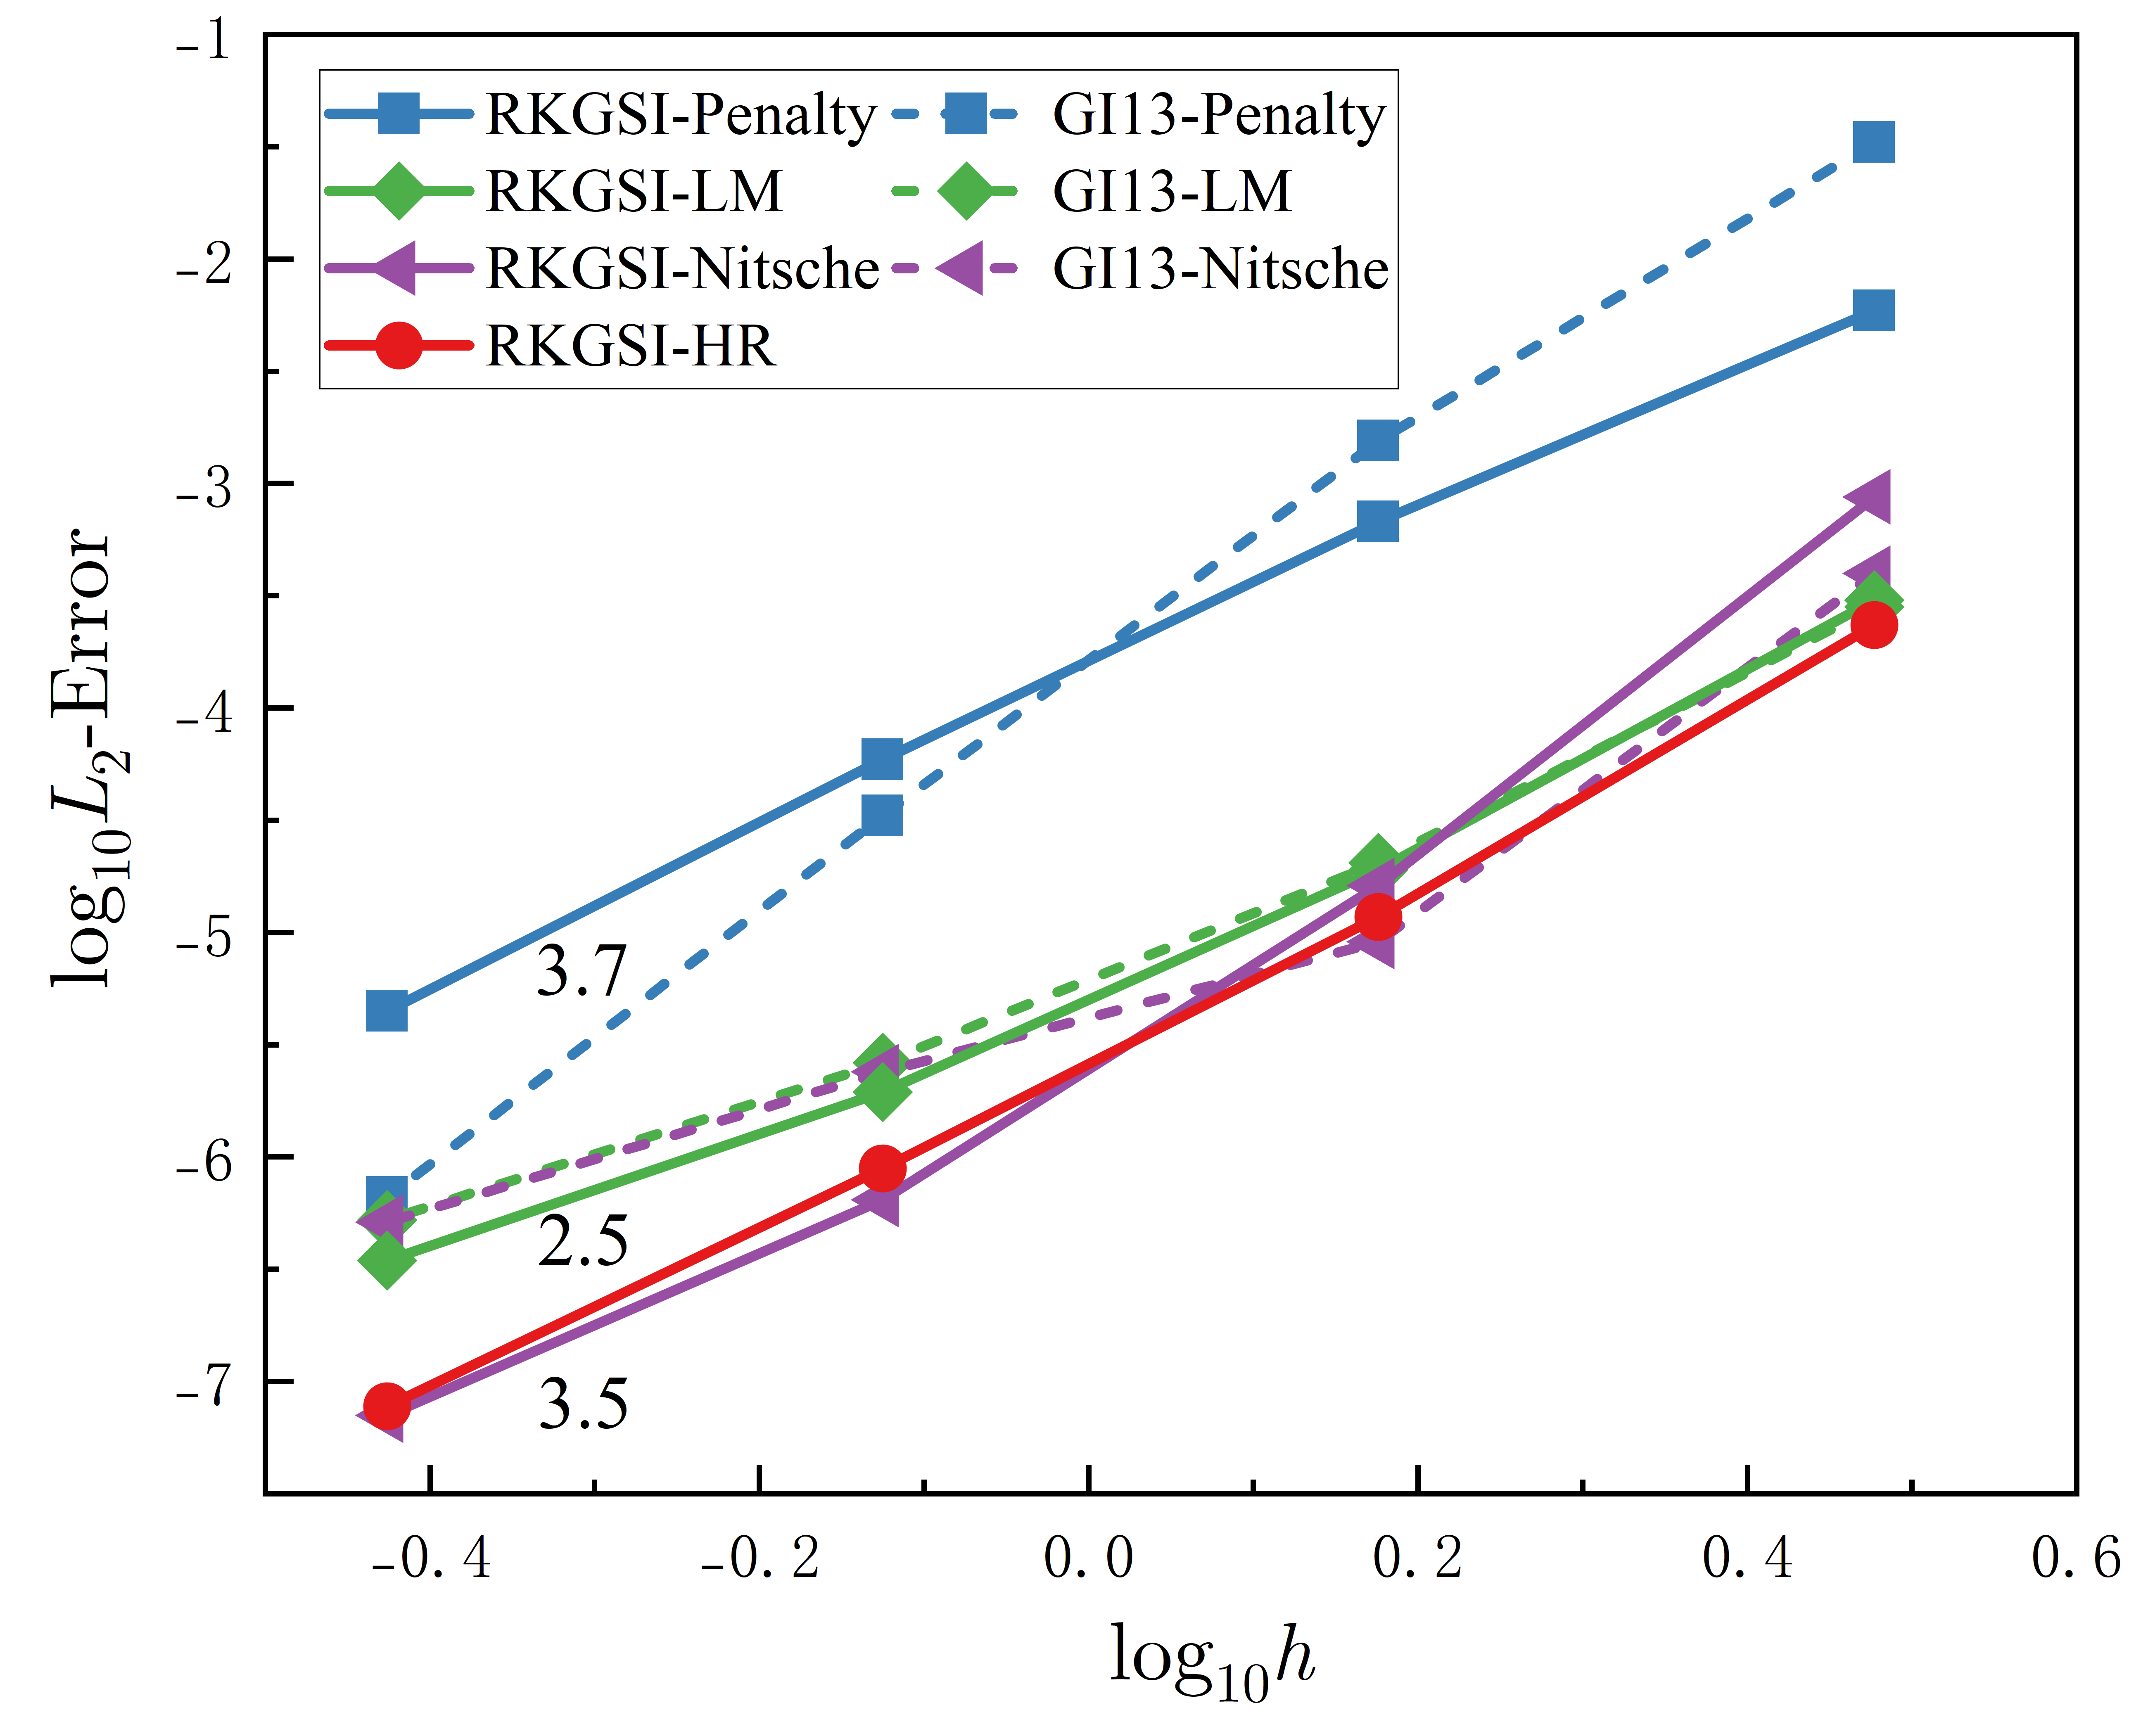
\includegraphics[scale=0.5]{figure/E/cantilever/L2.png}
    \caption{悬臂梁问题位移误差对比}\label{CL2}
\end{figure}
\begin{figure}[H]
    \centering
    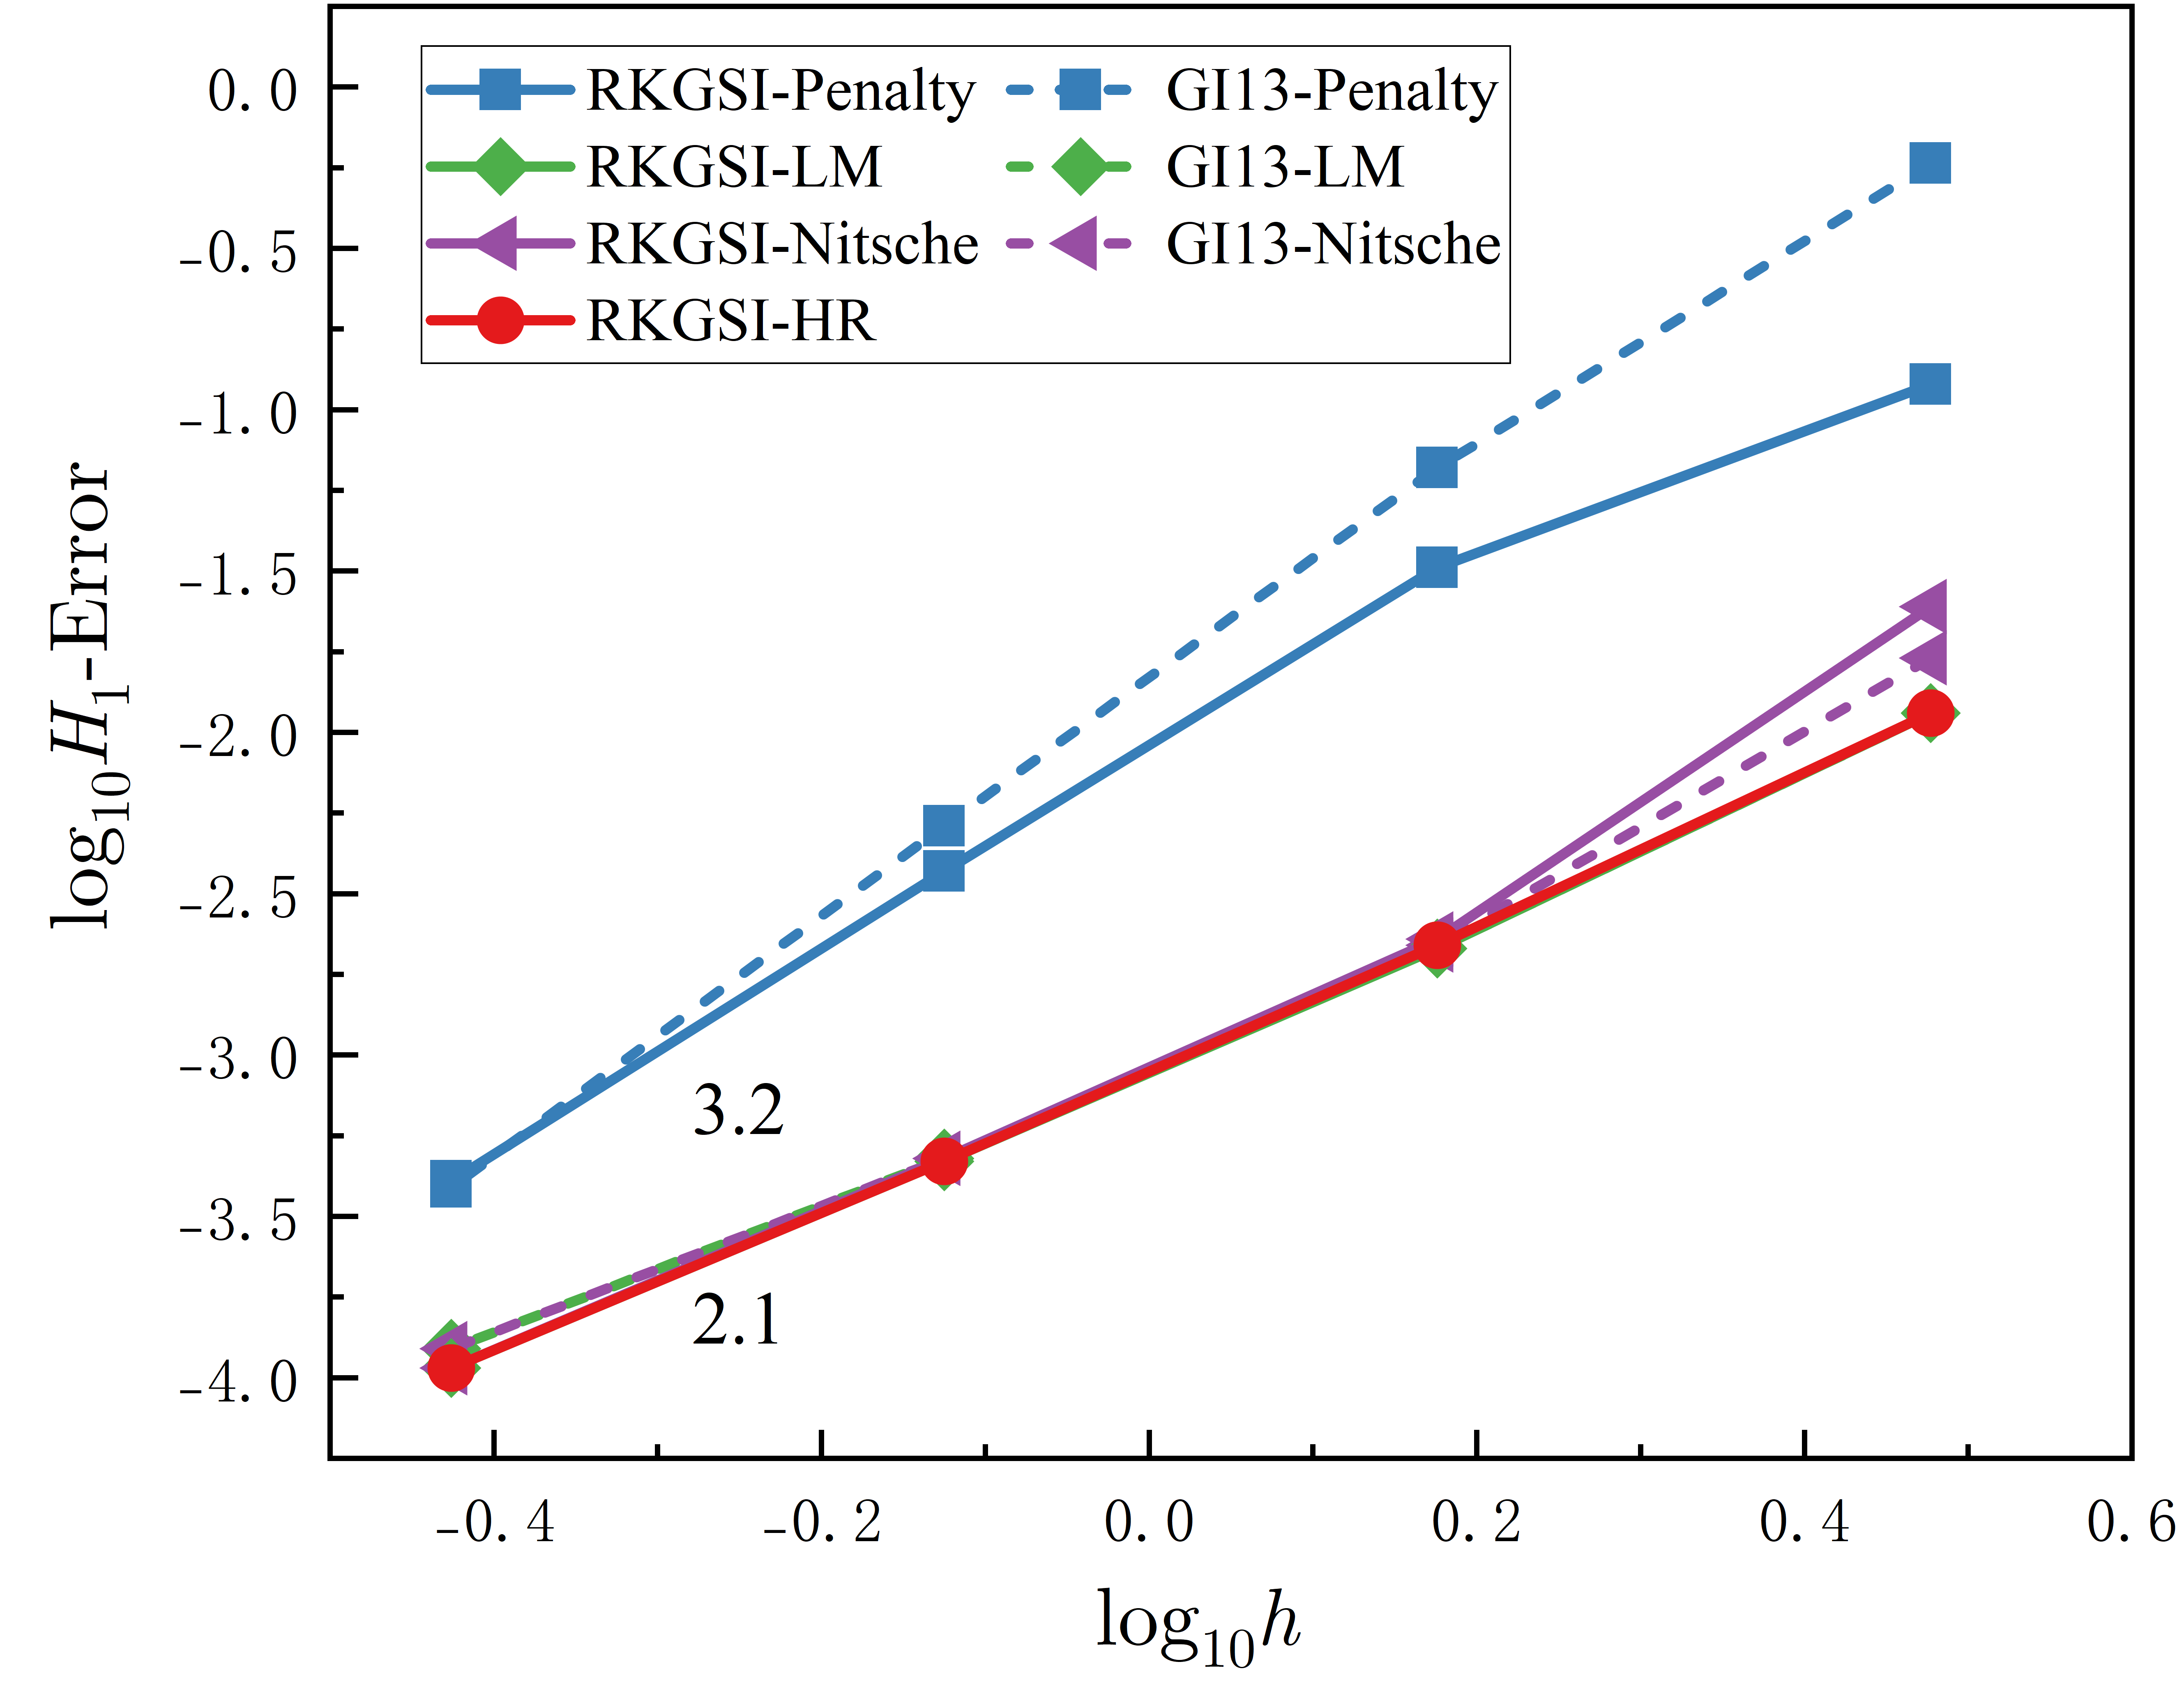
\includegraphics[scale=0.5]{figure/E/cantilever/H1.png}
    \caption{悬臂梁问题能量误差对比}\label{CH1}
\end{figure}
% 图(\ref{CCPUTime})为悬臂梁问题的节点数和计算时间的效率对比图。
% 从整体来看采用再生光滑梯度积分法(RKGSI)的计算效率明显高于传统高斯积分法(GI)。\par
\begin{figure}[H]
    \centering
    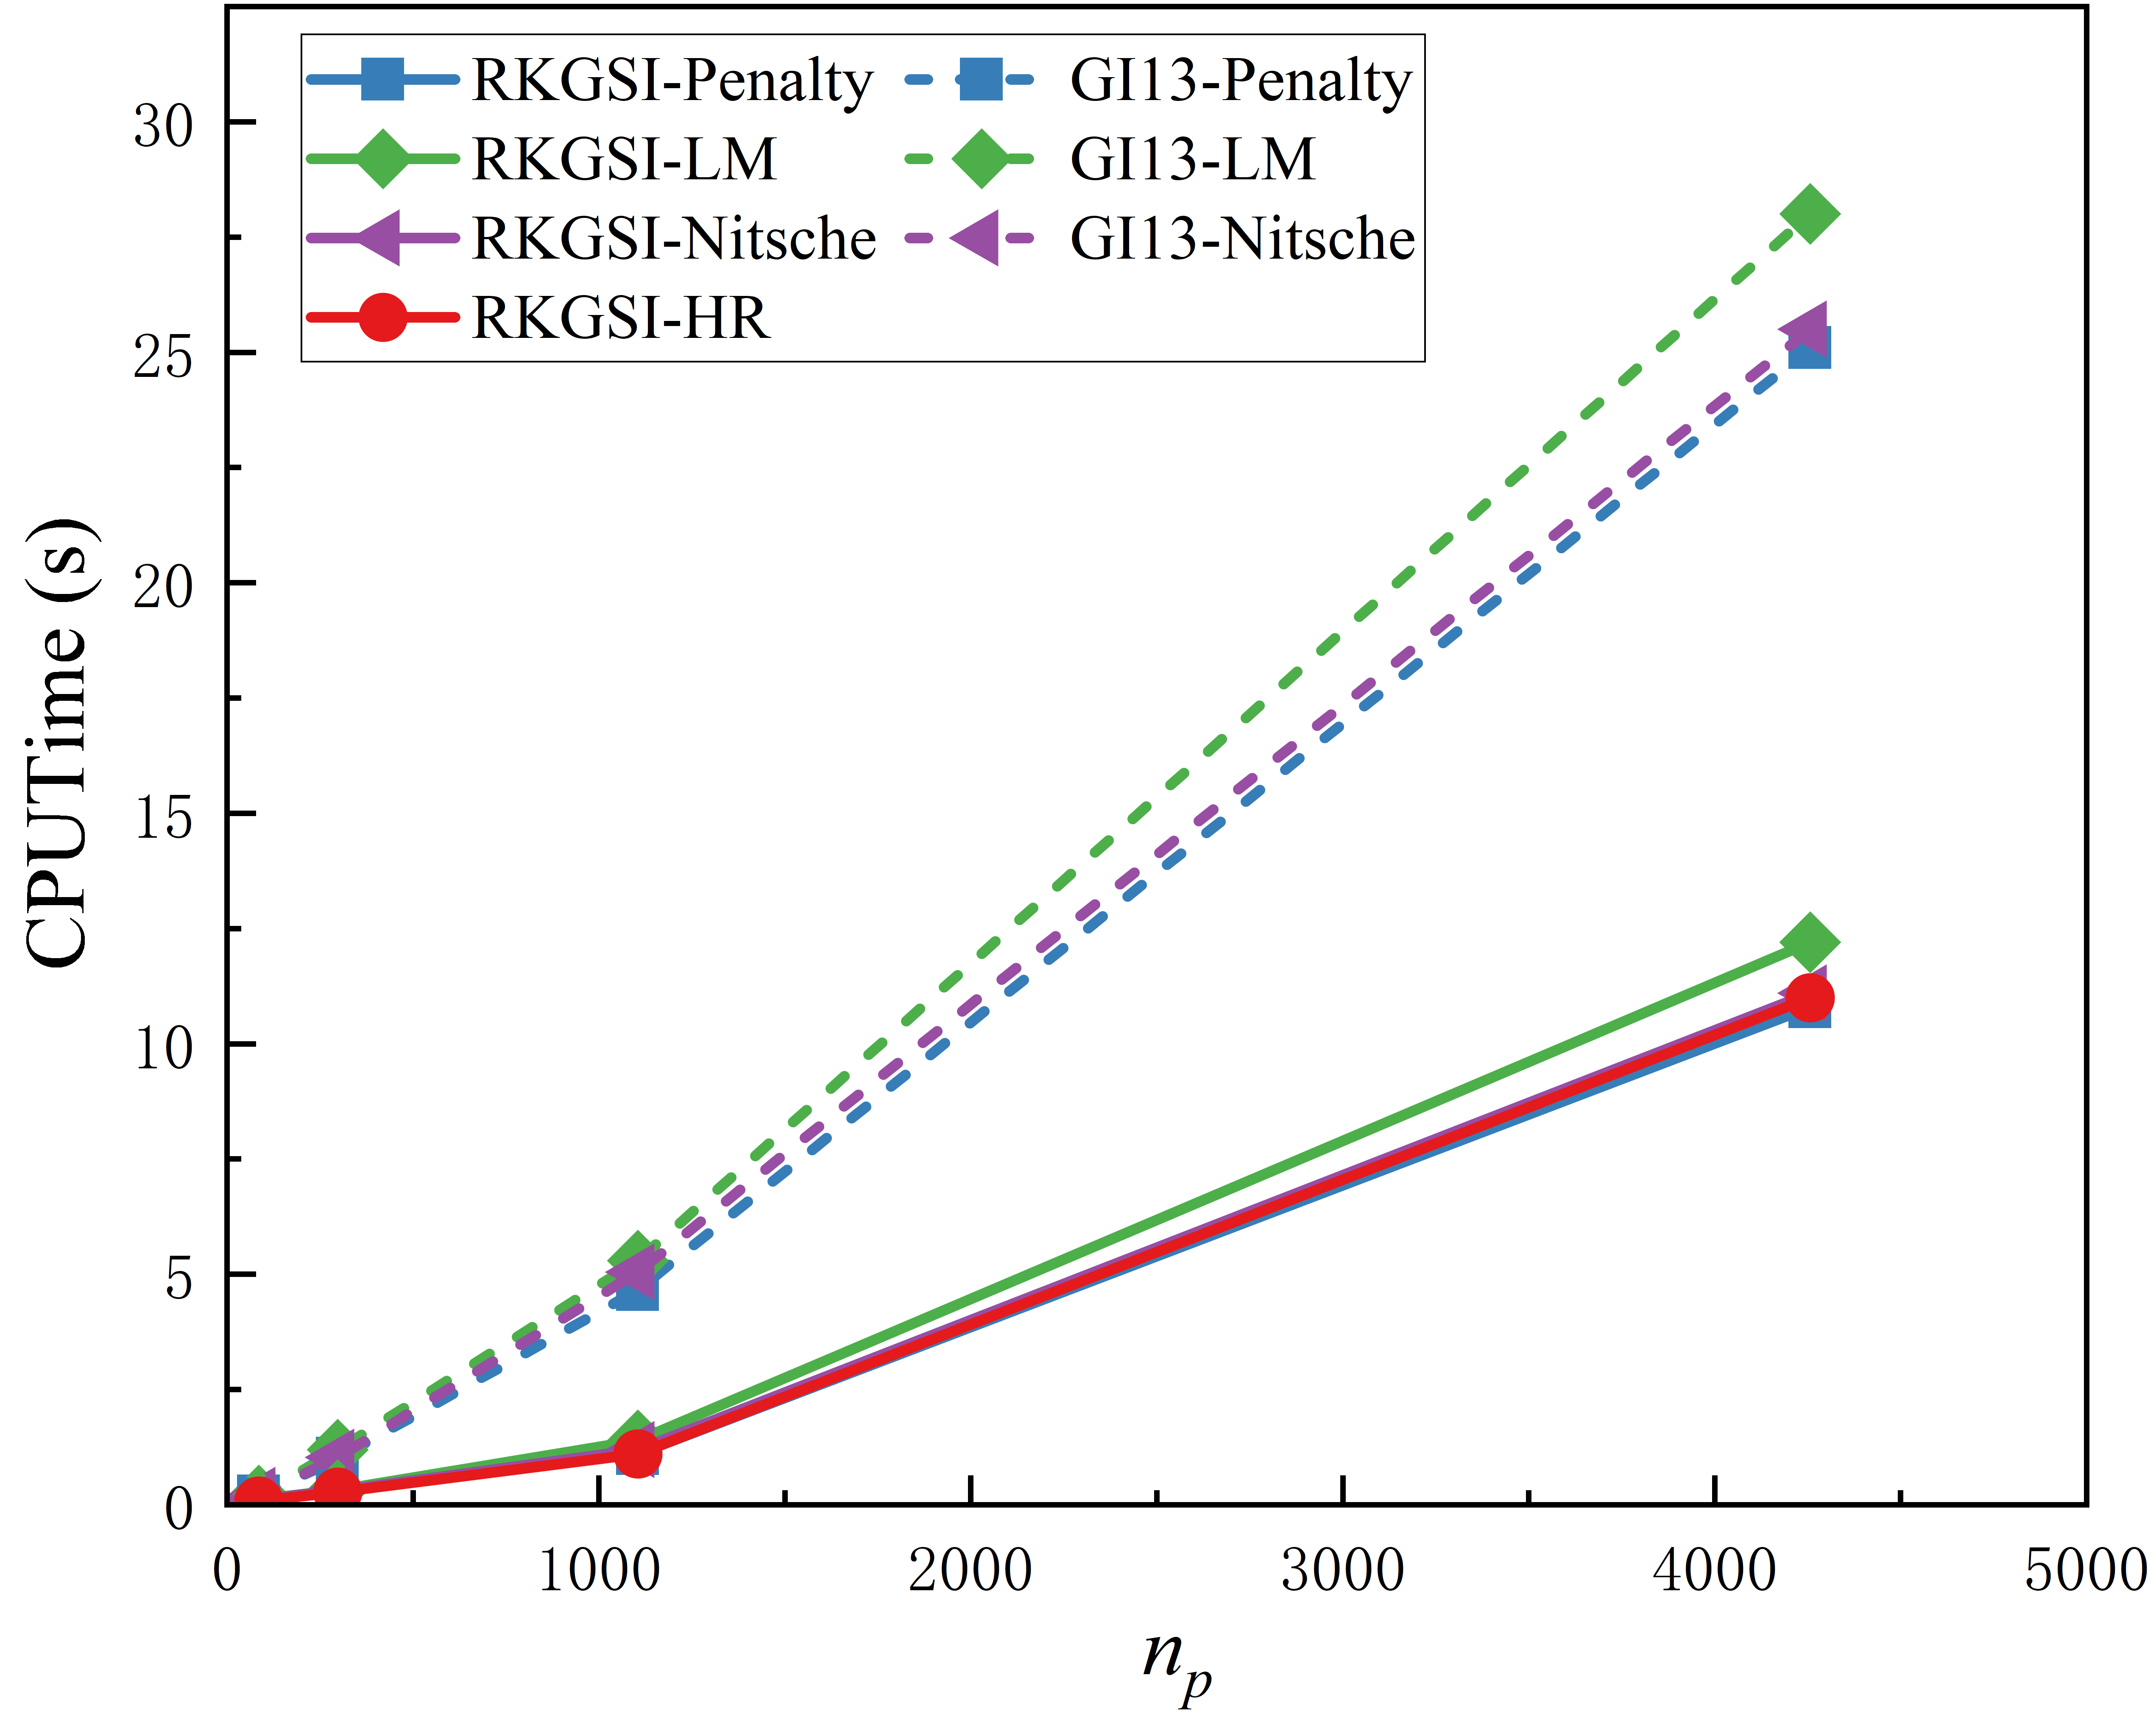
\includegraphics[scale=0.5]{figure/E/cantilever/CPUTime.png}
    \caption{计算时间与节点数的关系}\label{CCPUTime}
\end{figure}
% 图(\ref{Ccaculate})为悬臂梁问题的本质边界条件施加效率分析图。该图为施加强制边界$\Gamma^g$过程中计算形函数及梯度和组装相对应的刚度矩阵和力向量所用时间对比图。
% 从图中可以看出,罚函数法和拉格朗日乘子法在计算形函数及其梯度所用的时间相同且所用时间最少,这是由于罚函数法和拉格朗日乘子法在计算过程中只需要计算无网格形函数本身,无需计算无网格形函数梯度,
% 而Nitsche法和HR法也无需计算无网格形函数梯度,但需要计算再生光滑梯度,Nitshce法这部分所用的时间是罚函数法和拉格朗日乘子法的5.6倍,而HR法是1.6倍,HR法的计算效率高于Nitsche法。
% 组装相应的刚度矩阵和力向量这部分所用的时间上,Nitshe法和HR法计算效率基本相同。
% 从整体上来看,拉格朗日乘子法和罚函数法的效率优于HR法和Nitsche法,但拉格朗日乘子法和罚函数法不具有变分一致性无法达到理论误差收敛率。
% 因此,总体来说,相较于传统的本质边界条件施加方法,基于Hellinger-Reissner变分原理的本质边界条件施加方法(RKGSI-HR)能够达到理论误差收敛率,有效提高计算精度,相较于Nitsche法而言计算效率也更高。
% 
\begin{figure}[H]
    \centering
    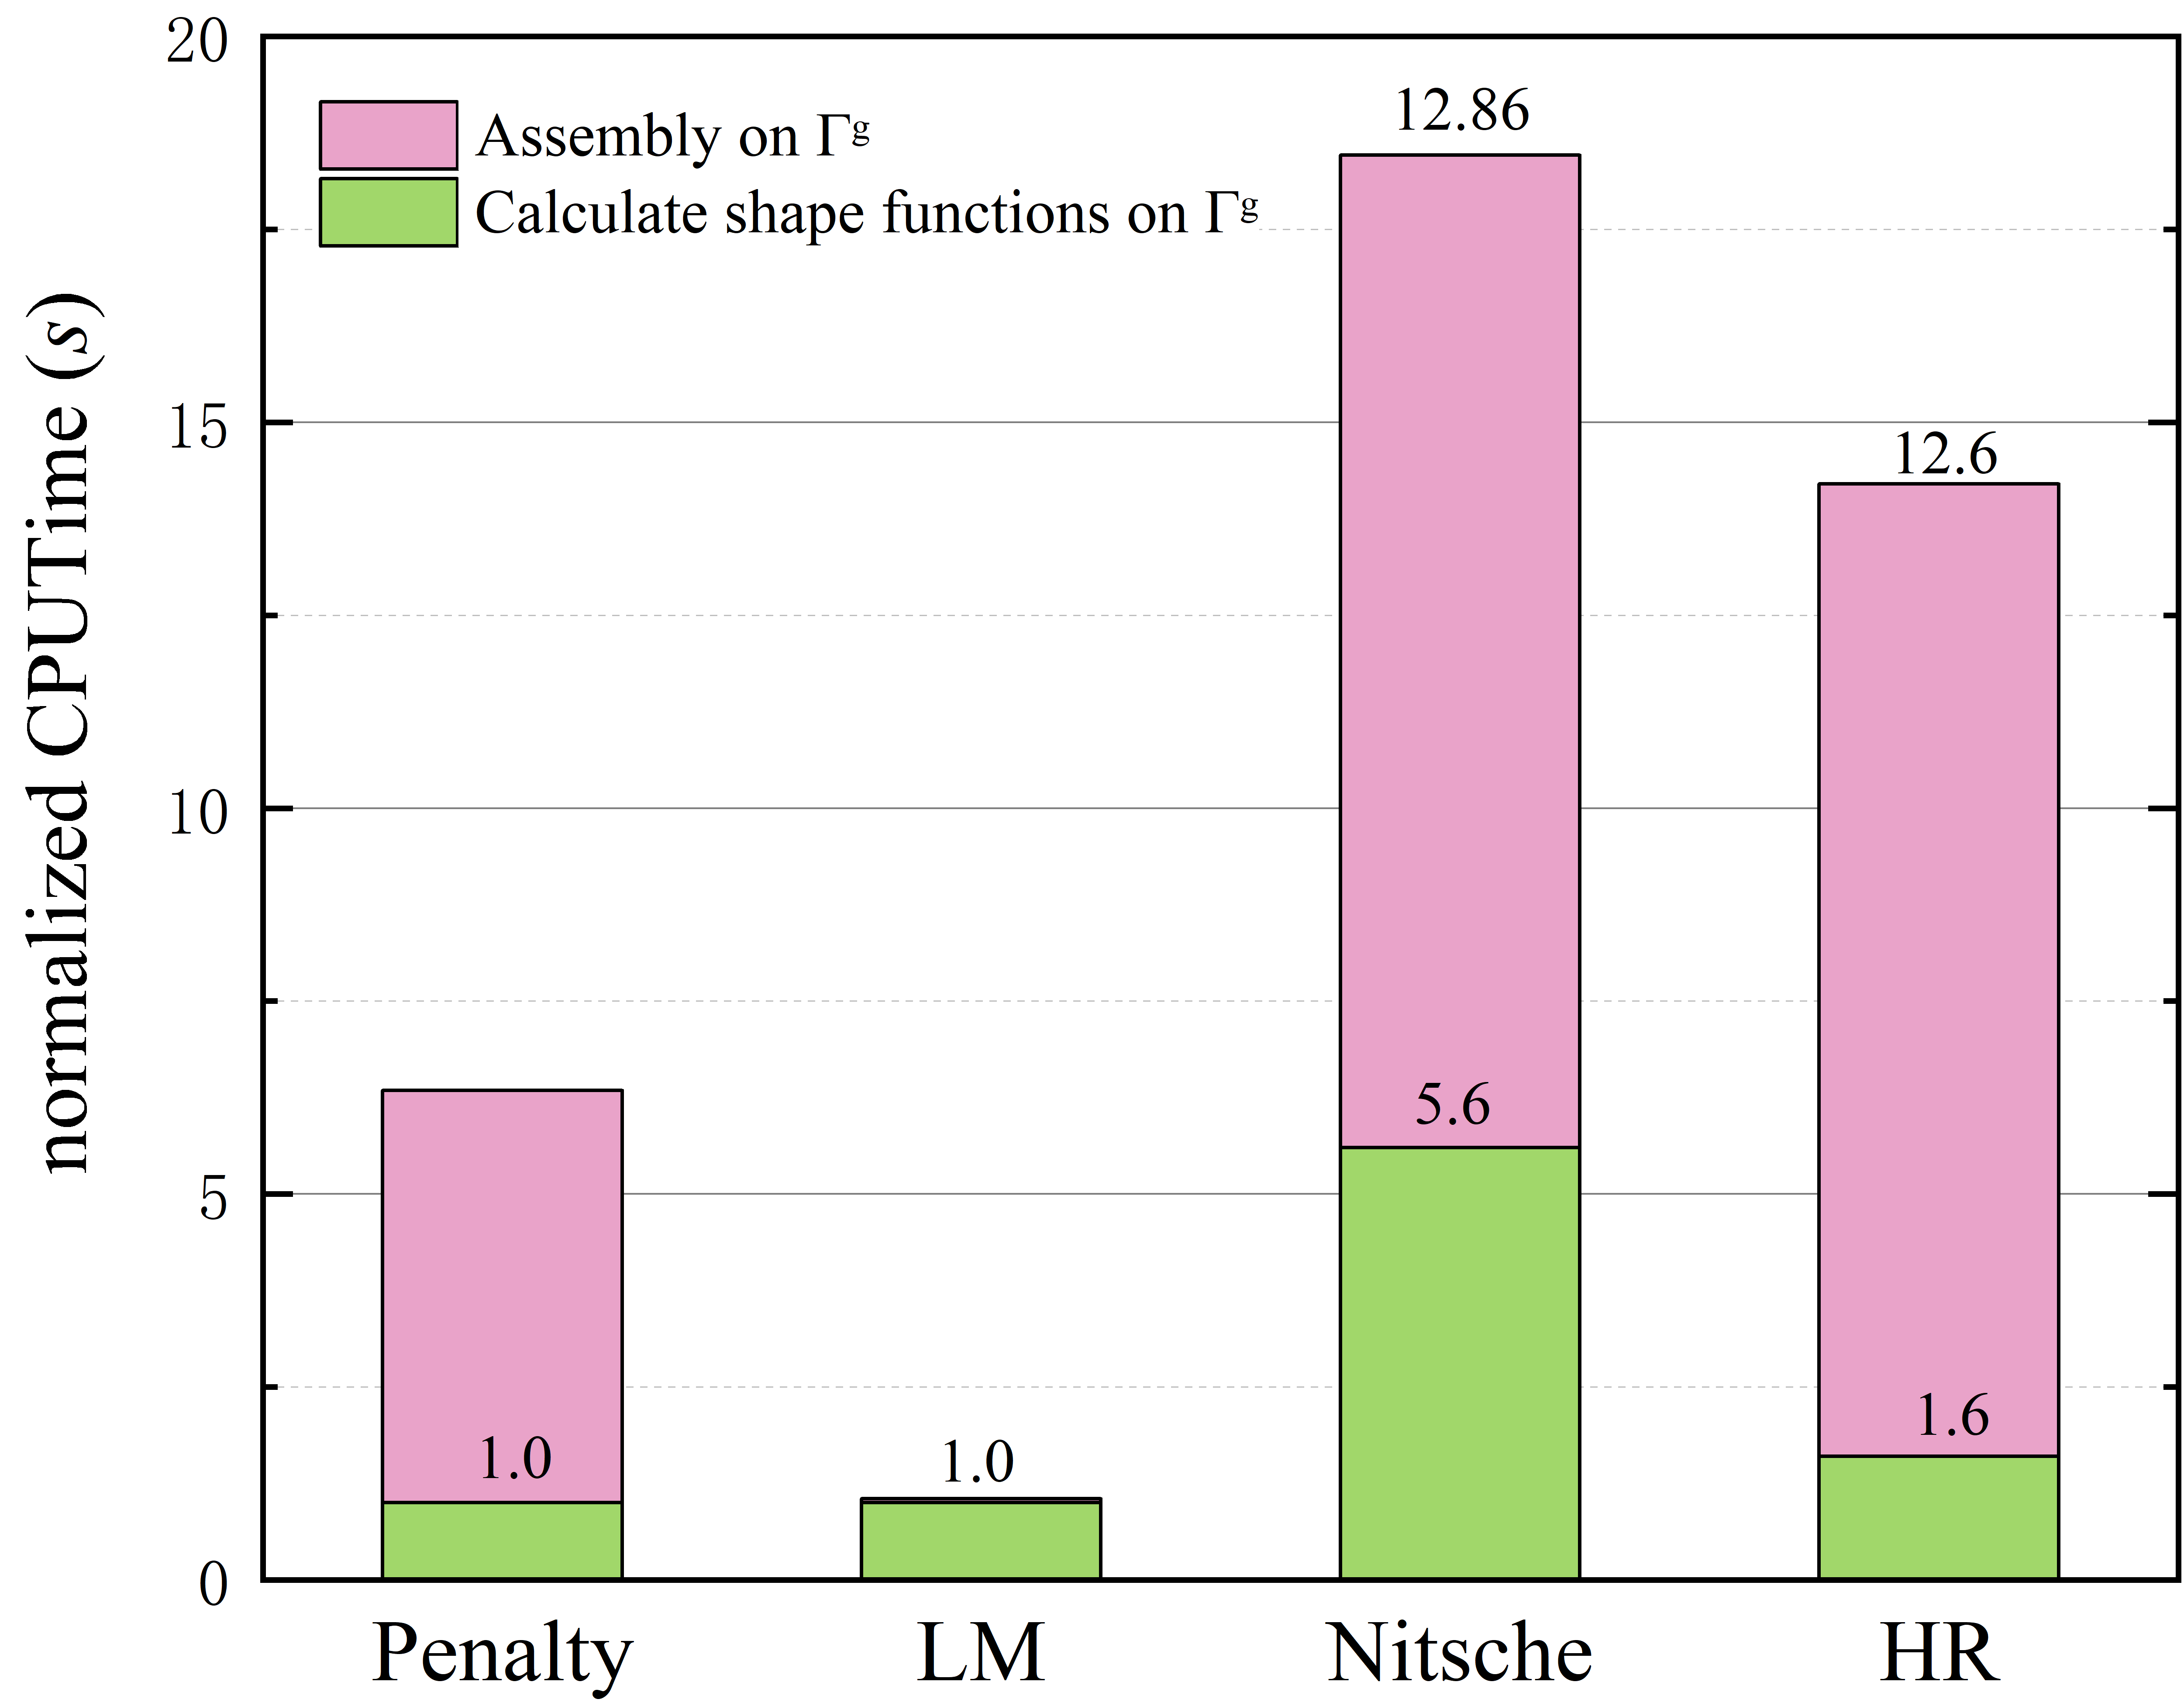
\includegraphics[scale=0.5]{figure/E/cantilever/caculate.png}
    \caption{本质边界条件施加效率分析}\label{Ccaculate}
\end{figure}
\subsection{带孔无限大平板问题}
考虑经典的带孔无限大平板问题,如图(\ref{hole})所示,板的的中心存在一半径为$a=1$的圆形小孔,同时平板的无穷远处沿$x$轴方向施加均布荷载$T=1000$。
板的材料系数为杨氏模量$E=3\times10^6$、泊松比$\nu=0.3$。根据Michell解可以得到该带孔无限大平板问题的解析解为:
\begin{equation}
\begin{split}
\begin{cases}
    u_x(r,\theta)=\frac{Ta}{8\mu}(\frac{r}{a}(k+1)cos\theta-\frac{2a^3}{r^3}cos3\theta+\frac{2a}{r}((1+k)cos\theta+cos3\theta))\\
    u_y(r,\theta)=\frac{Ta}{8\mu}(\frac{r}{a}(k-3)sin\theta-\frac{2a^3}{r^3}sin3\theta+\frac{2a}{r}((1-k)sin\theta+sin3\theta))  
\end{cases}
\end{split}
\end{equation}
其中,$k$和$\mu$分别为:
\begin{equation}
\begin{split}
    k=\frac{3-\nu}{1+\nu}\quad \text{,}\mu=\frac{E}{2(1+\nu)}
\end{split}
\end{equation}
与之相对应的应力分量为:
\begin{equation}
\begin{split}
\begin{cases}
    \sigma_{xx}=T(1-\frac{a^2}{r^2}(\frac{3}{2}cos2\theta+cos4\theta)+\frac{3a^4}{2r^4}cos4\theta)\\
    \sigma_{yy}=-T(\frac{a^2}{r^2}(\frac{1}{2}cos2\theta-cos4\theta)+\frac{3a^4}{2r^4}cos4\theta)\\
    \sigma_{xy}=-T(\frac{a^2}{r^2}(\frac{1}{2}sin2\theta+sin4\theta)-\frac{3a^4}{2r^4}sin4\theta)\\
\end{cases}
\end{split}
\end{equation}\par
如图(\ref{hole})所示,根据带孔无限大平板的对称性,取边长$b=5$的四分之一的方形域作为研究对象。
方形域的上端和右端以及圆孔的边界施加自然边界条件$\Gamma^t$,而方形域的左端和下端约束法向位移,施加强制边界条件$\Gamma^g$。
该求解域分别通过图(\ref{hole.msh})所示采用$\text{(a)}112$、$\text{(b)}403$、$\text{(c)}1525$、$\text{(d)}5929$的四个疏密不同的节点进行离散。
对于采用三次基函数的带孔无限大平板算例问题,传统高斯积分法采用16点高斯积分,核函数的相对影响域为3.5。\par
\begin{figure}[H]
\centering
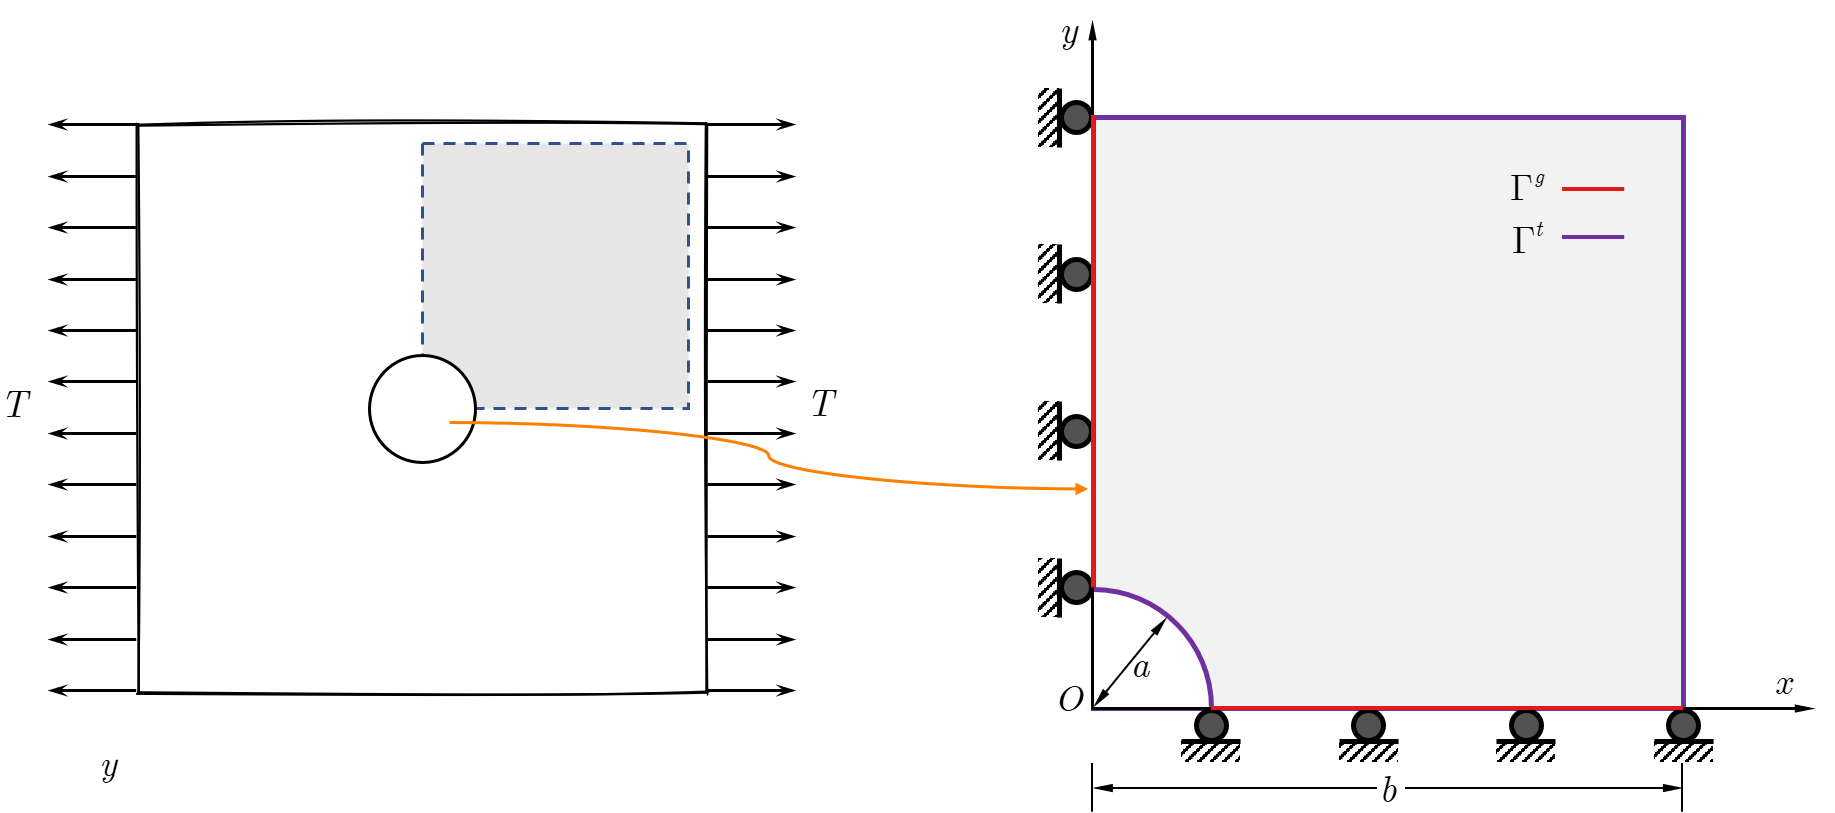
\includegraphics[scale=0.5]{figure/E/hole/hole.png}
    \caption{带孔无限大平板问题模型}\label{hole}
\end{figure}
\begin{figure}
\centering
 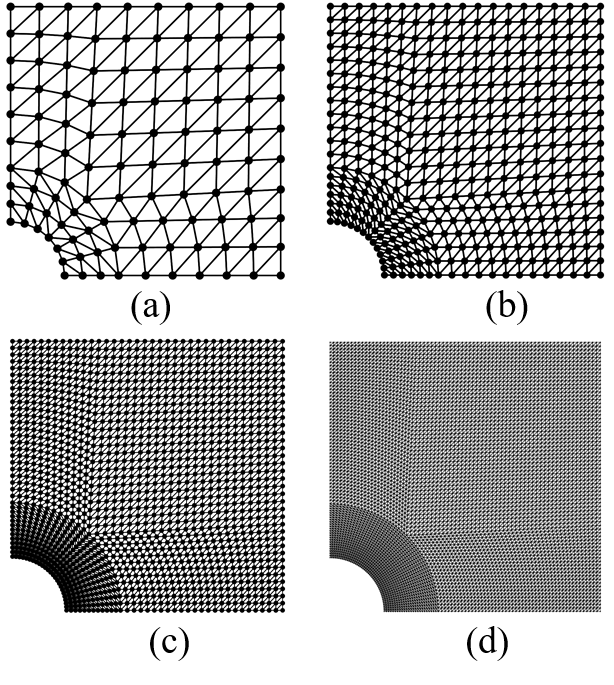
\includegraphics[scale=0.7]{figure/E/hole/hole.msh.png}
   \caption{带孔无限大平板问题无网格离散}\label{hole.msh}
\end{figure}
图(\ref{HL2})、(\ref{HH1})为带孔无限大平板问题的位移和能量误差对比图。
从图中可以看出传统高斯积分法由于不具有变分一致性,导致GI-Penalty法、GI-LM法、GI-Nistche法均无法达到理论误差收敛率。
基于Hellinger-Reissner变分原理的本质边界条件施加方法(RKGSI-HR)和RKGSI-Nitsche法满足变分一致性能够达到理论误差收敛率。
虽然RKGSI-LM法无法通过分片实验不满足变分一致性,但由于拉格朗日乘子法法具有较高的精度也能达到理论误差收敛率。
图(\ref{HCPUTime})、(\ref{Hcaculate})为带孔无限大平板问题的效率对比图。
从图中可以看出随着无网格节点数的增加,采用再生光滑梯度积分法(RKGSI)的效率明显高于传统高斯积分法(GI),在施加强制边界条件的过程中,HR法不仅满足变分一致性同时计算效率还高于传统的Nitsche法。
最后,图(\ref{Hstress})为带孔无限大平板问题的应力云图,从图中可以看出RKGSI-Penalty法和精确解之间是有差异的,
而RKGSI-Nitsche法和RKGSI-HR法是和精确解几乎相同。但Nitsche法是需要依靠人工经验参数并且计算效率也低于HR法。
\begin{figure}[H]
    \centering
    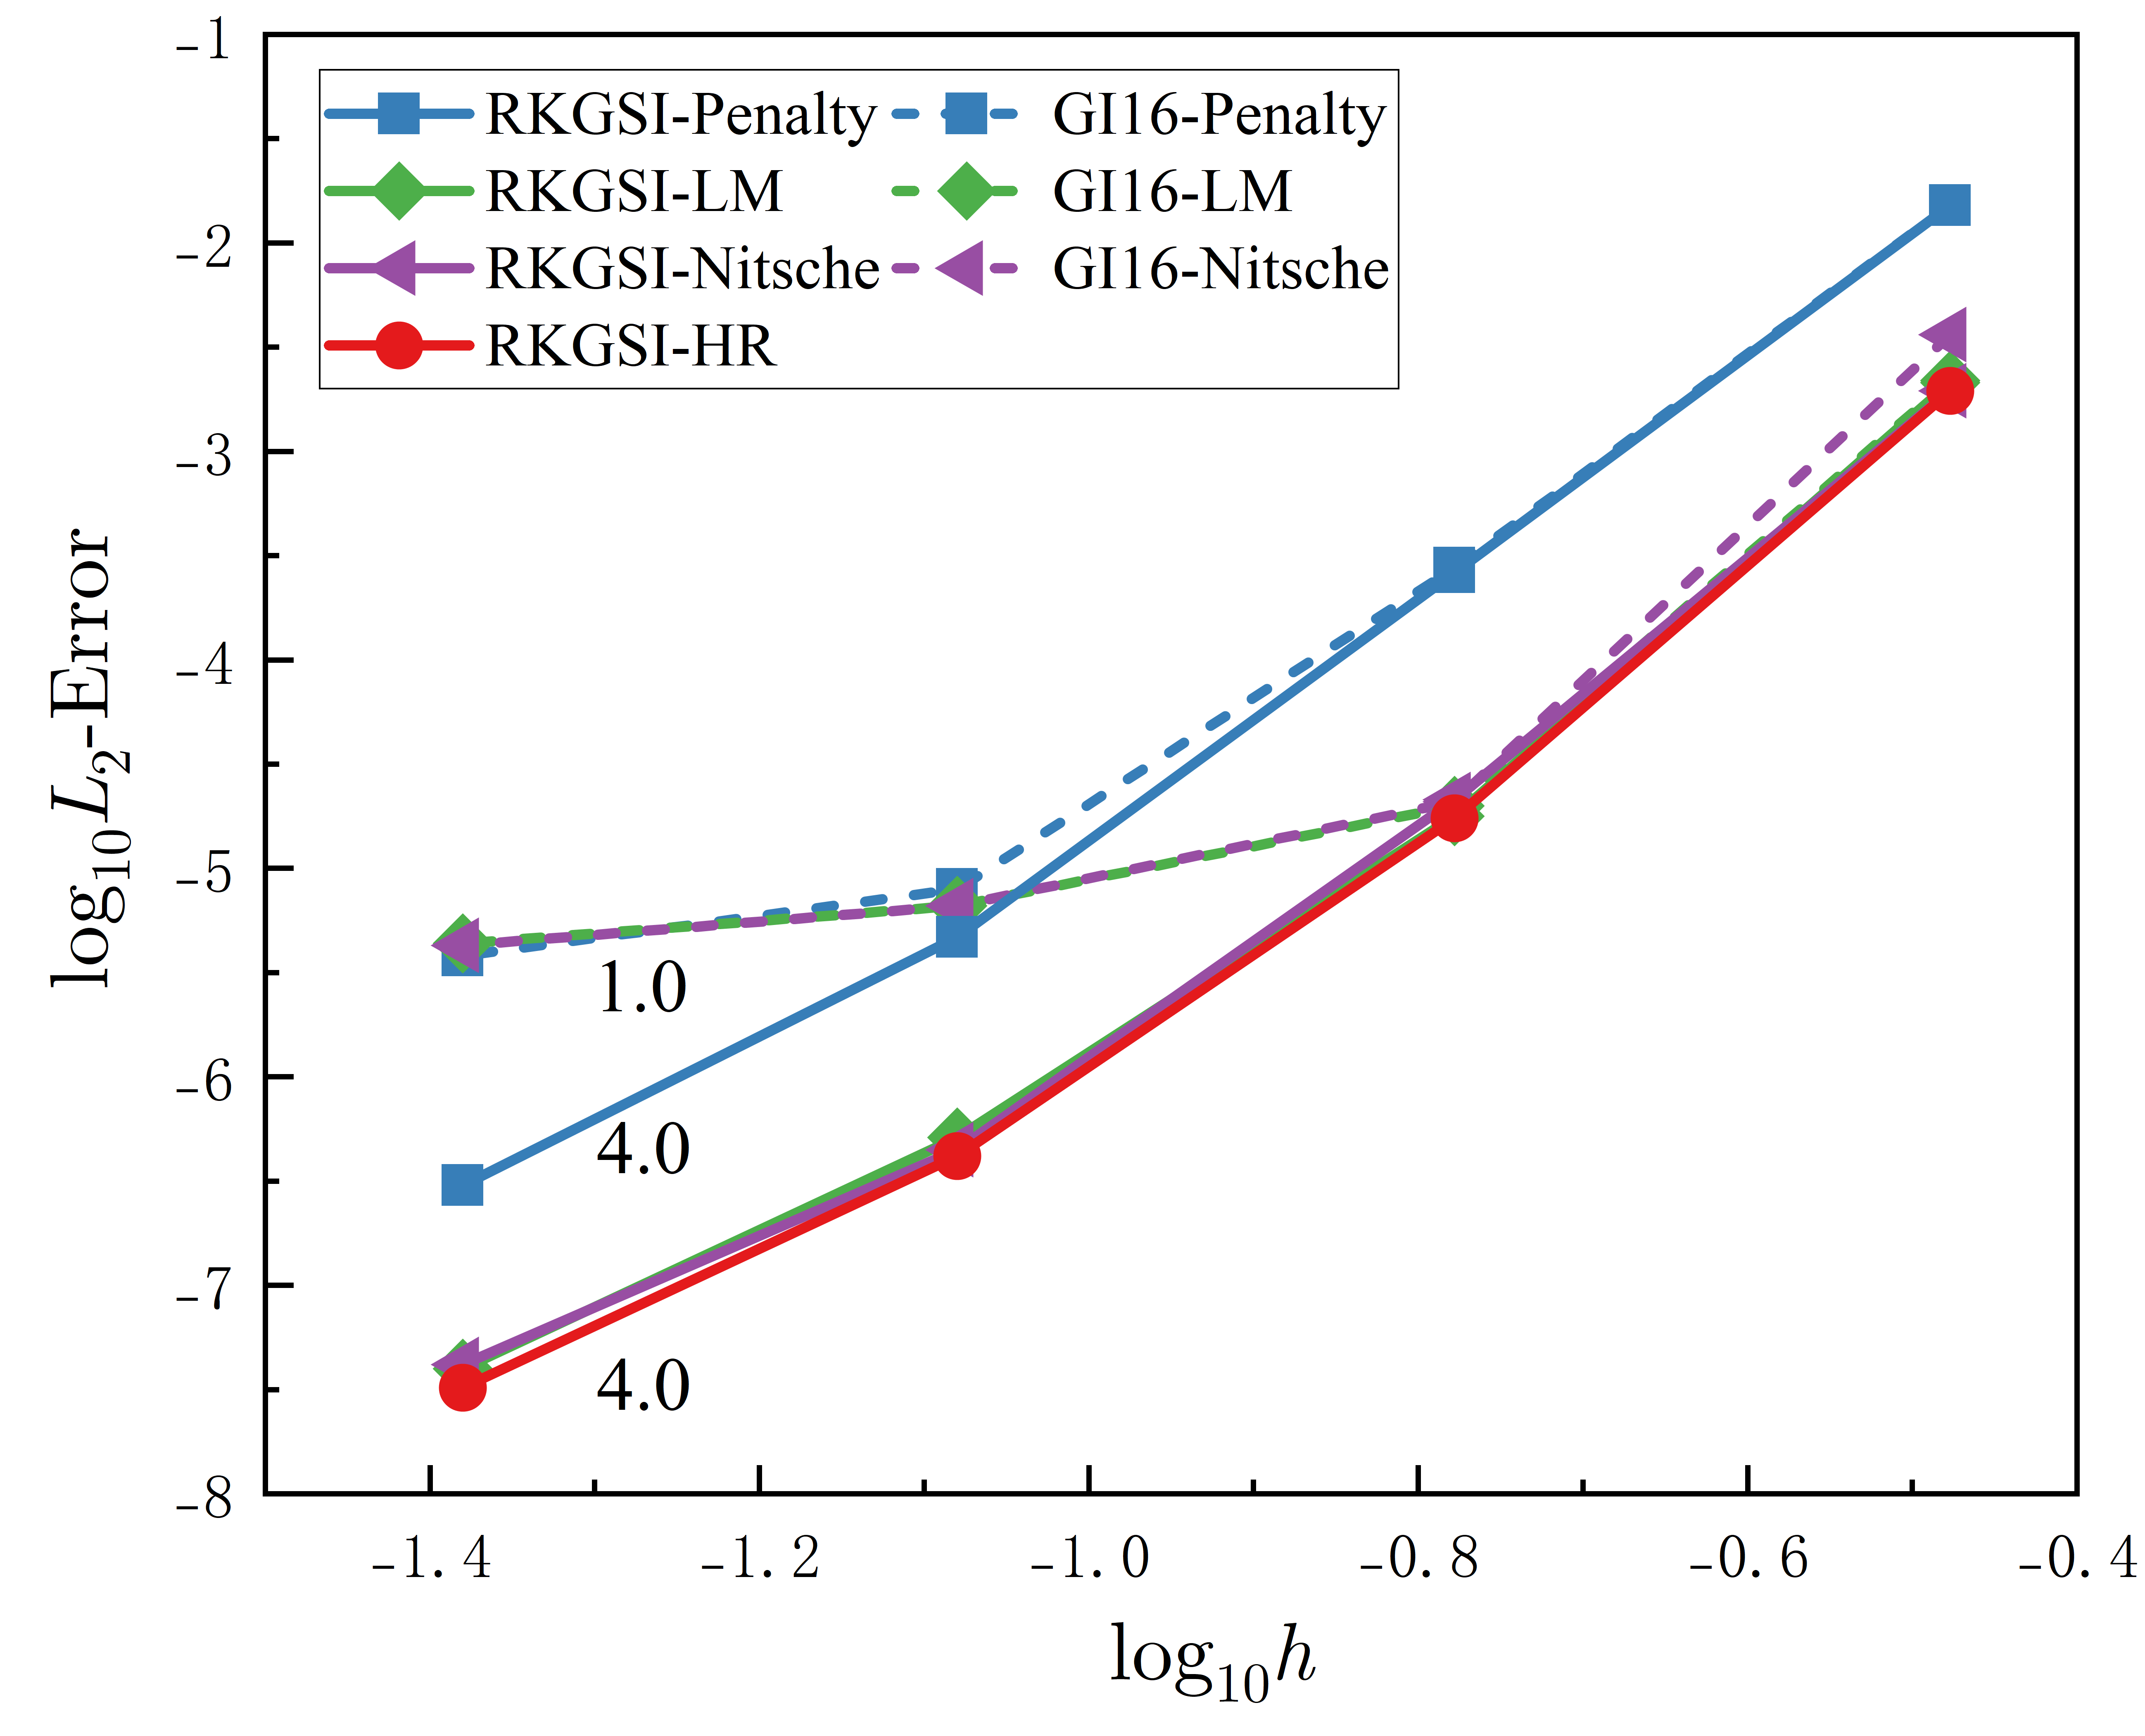
\includegraphics[scale=0.5]{figure/E/hole/L2.png}
    \caption{带孔无限大平板问题位移误差对比}\label{HL2}
\end{figure}
\begin{figure}[H]
    \centering
    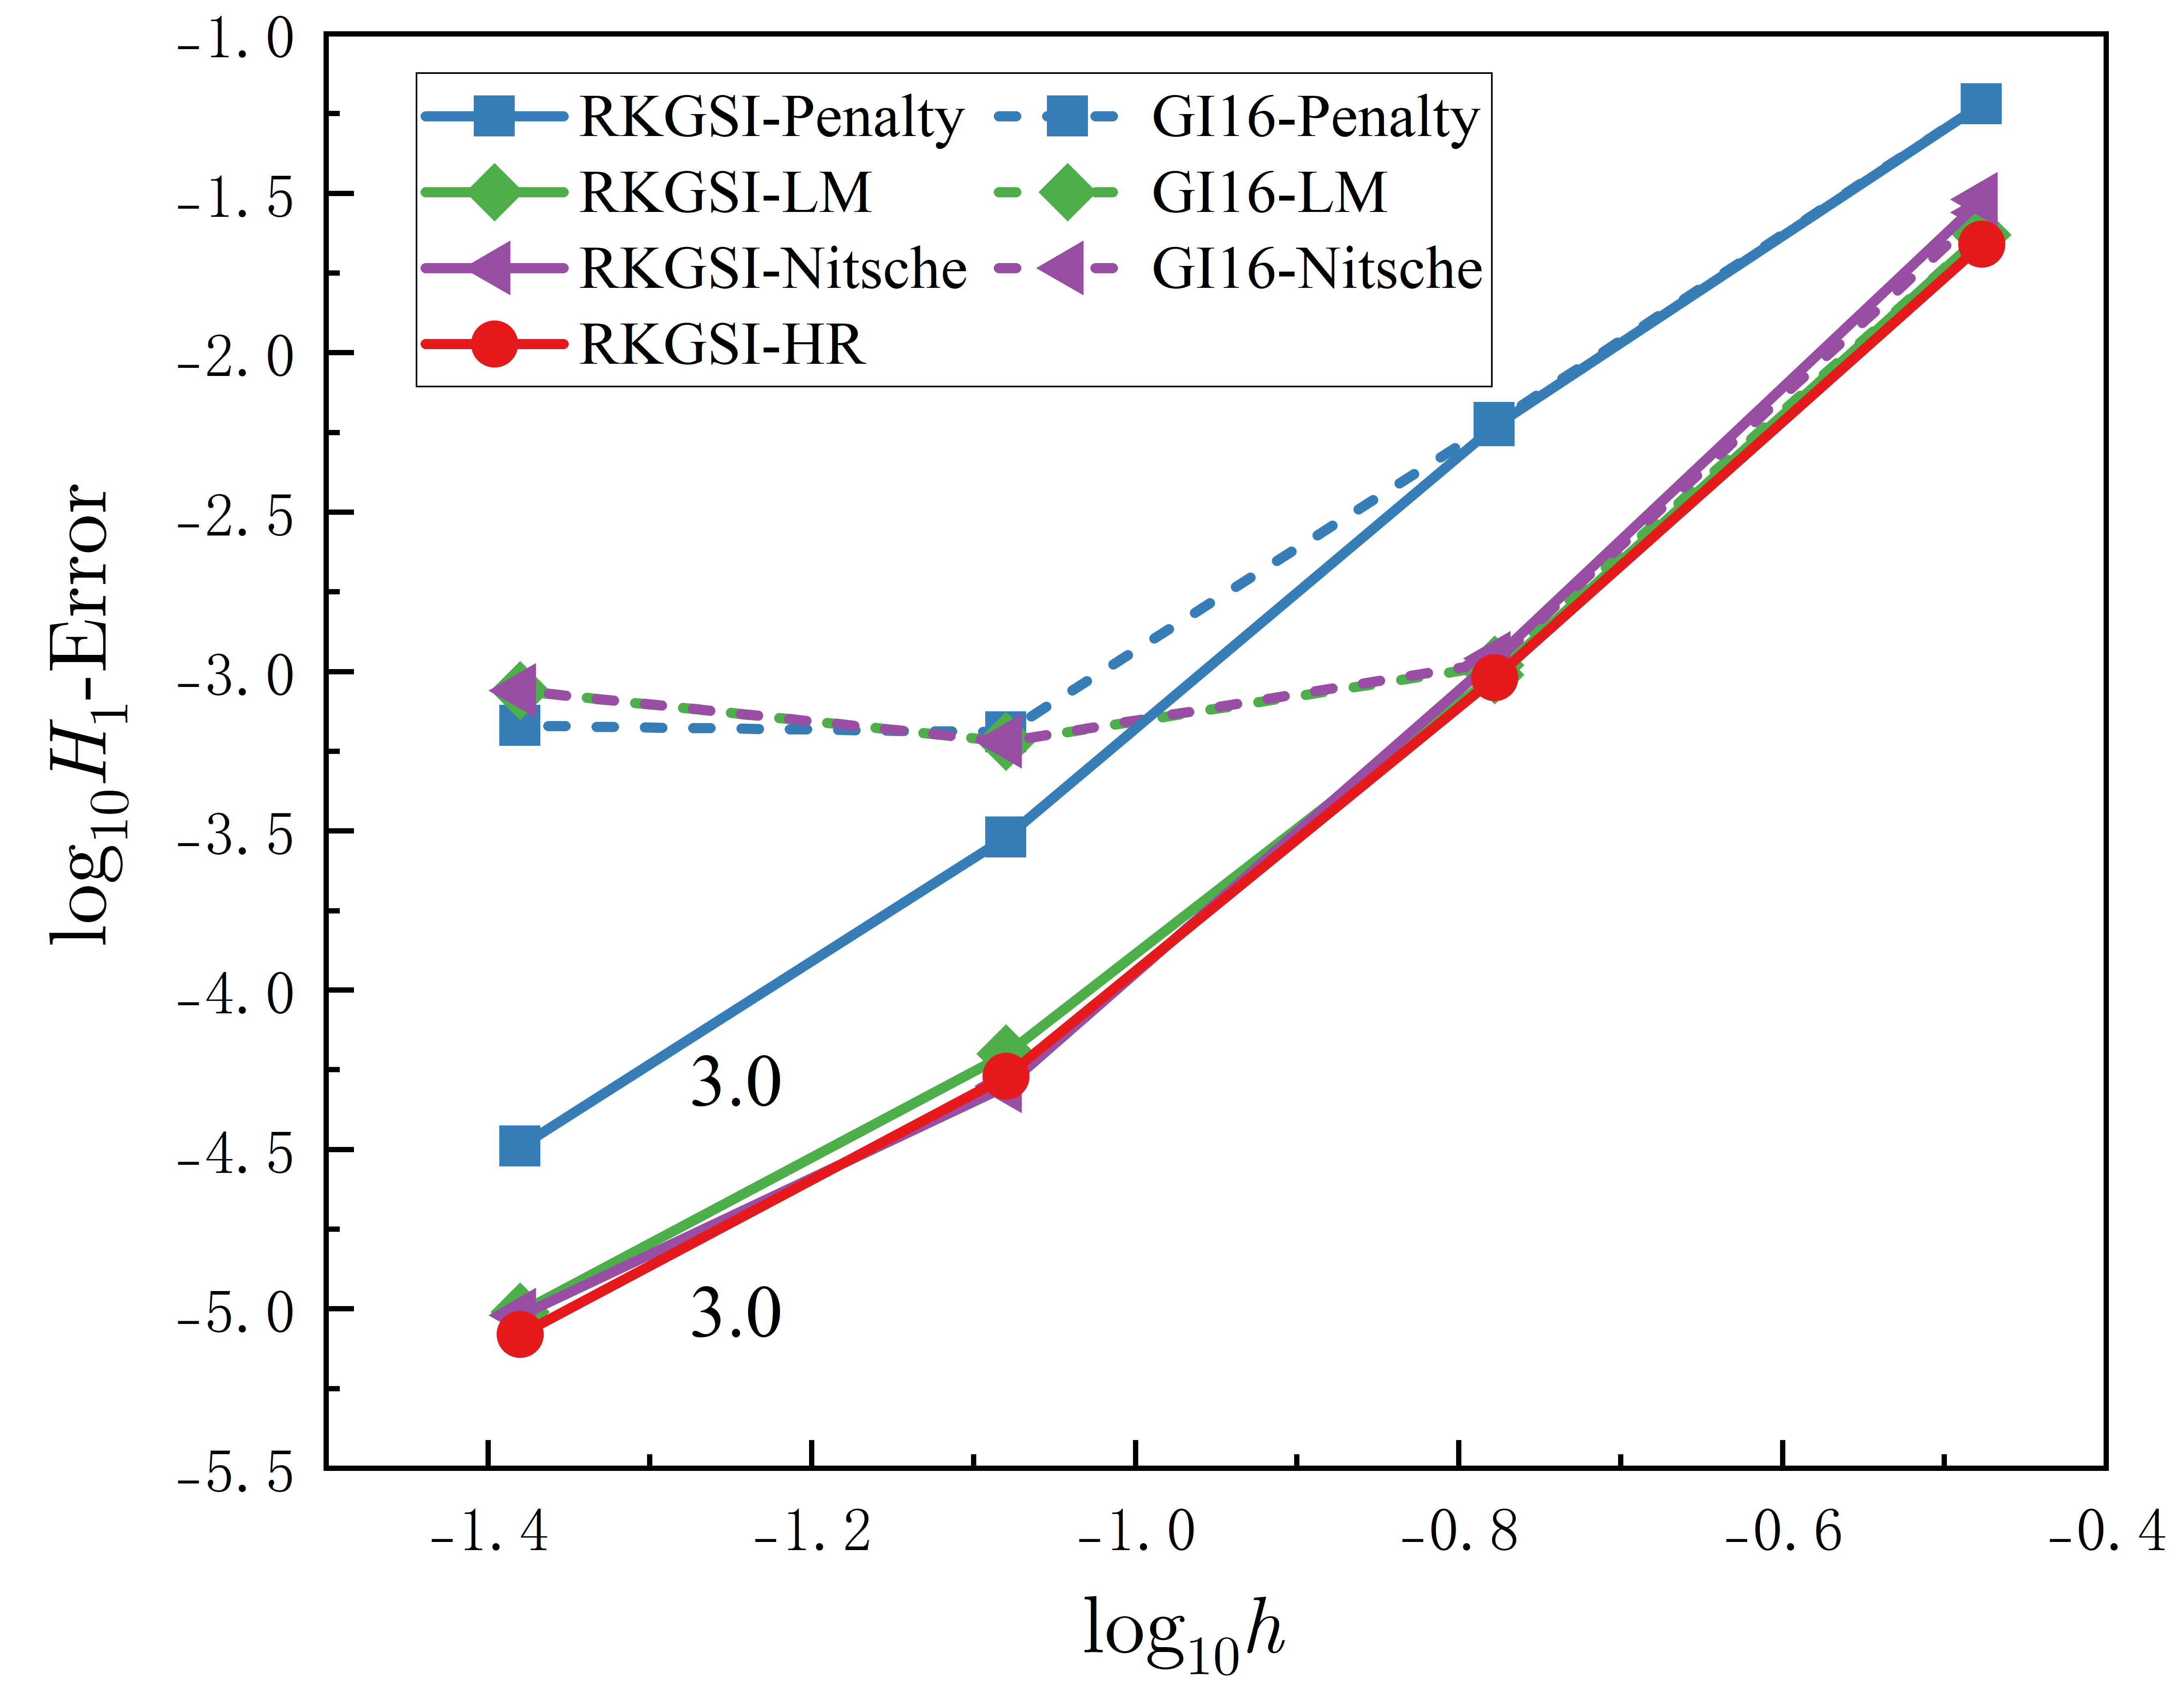
\includegraphics[scale=0.5]{figure/E/hole/H1.png}
    \caption{带孔无限大平板问题能量误差对比}\label{HH1}
\end{figure}
% 图(\ref{HCPUTime})、(\ref{Hcaculate})为带孔无限大平板问题的效率对比图。
% 从图中可以看出随着无网格节点数的增加,采用再生光滑梯度积分法(RKGSI)的效率明显高于传统高斯积分法(GI),在施加强制边界条件的过程中,HR法不仅满足变分一致性同时计算效率还高于传统的Nitsche法
% 
\begin{figure}[H]
    \centering
    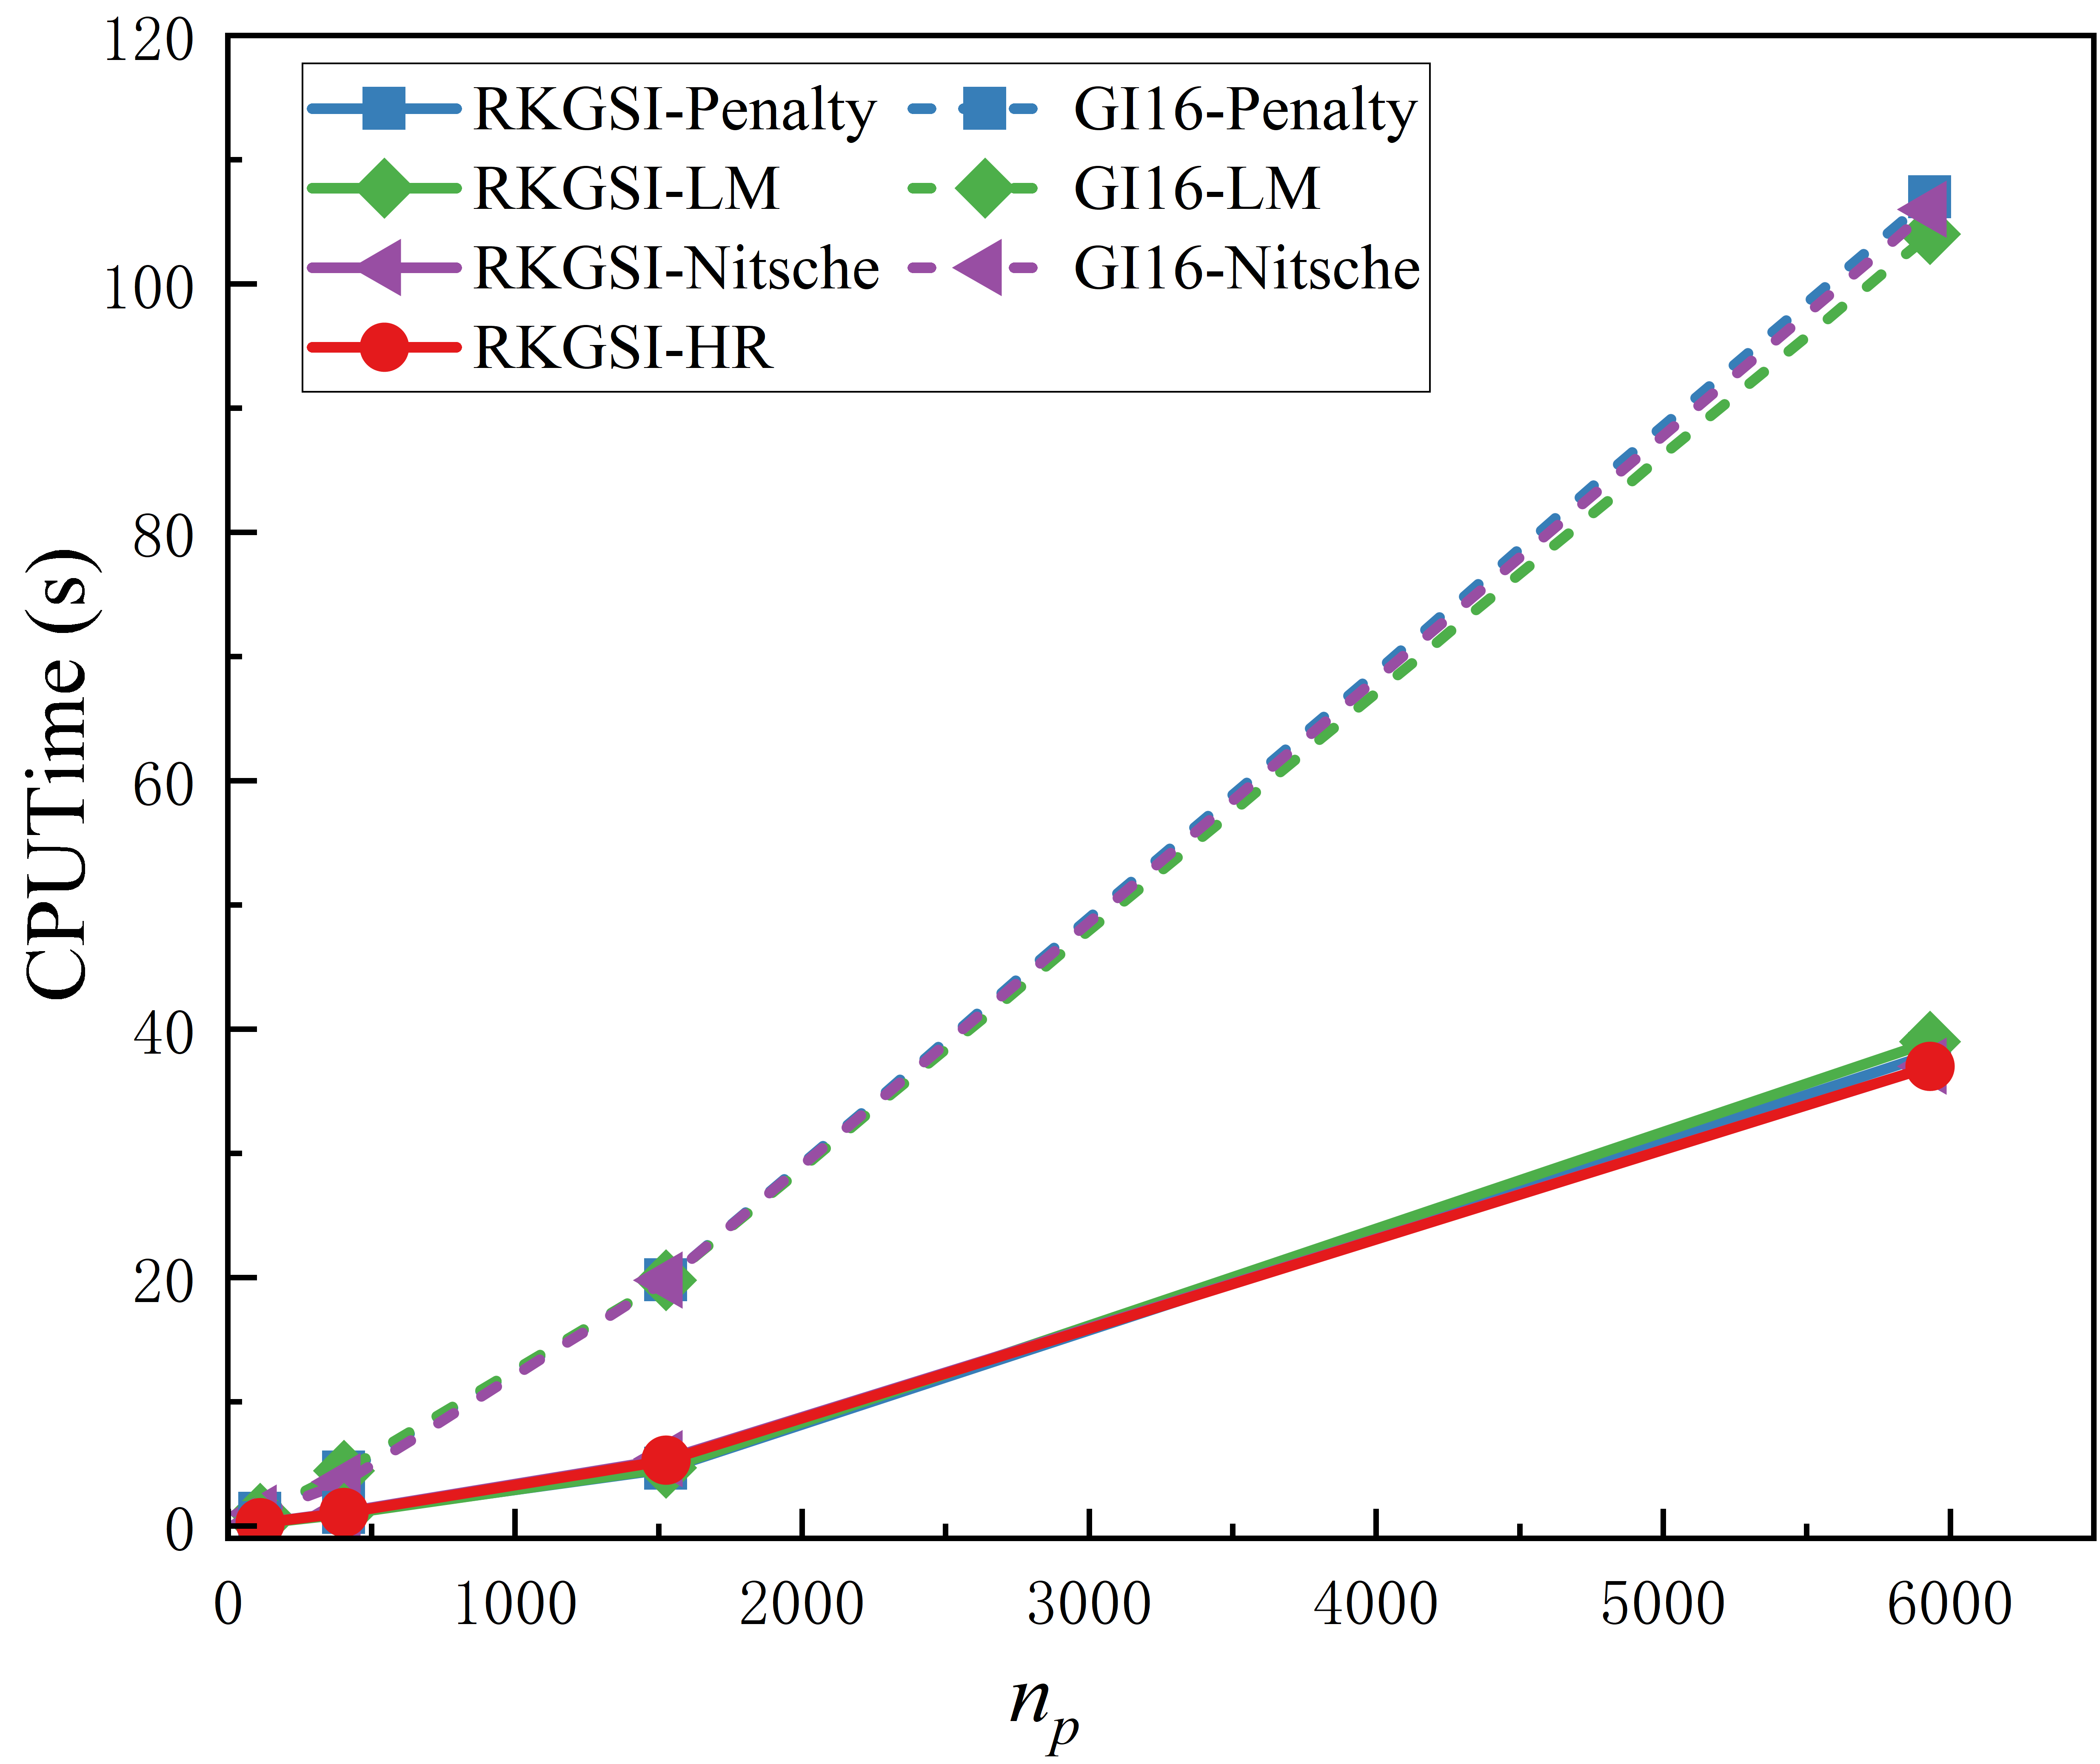
\includegraphics[scale=0.5]{figure/E/hole/CPUTime.png}
    \caption{带孔无限大平板问题计算时间与节点数关系}\label{HCPUTime}
\end{figure}
\begin{figure}[H]
    \centering
    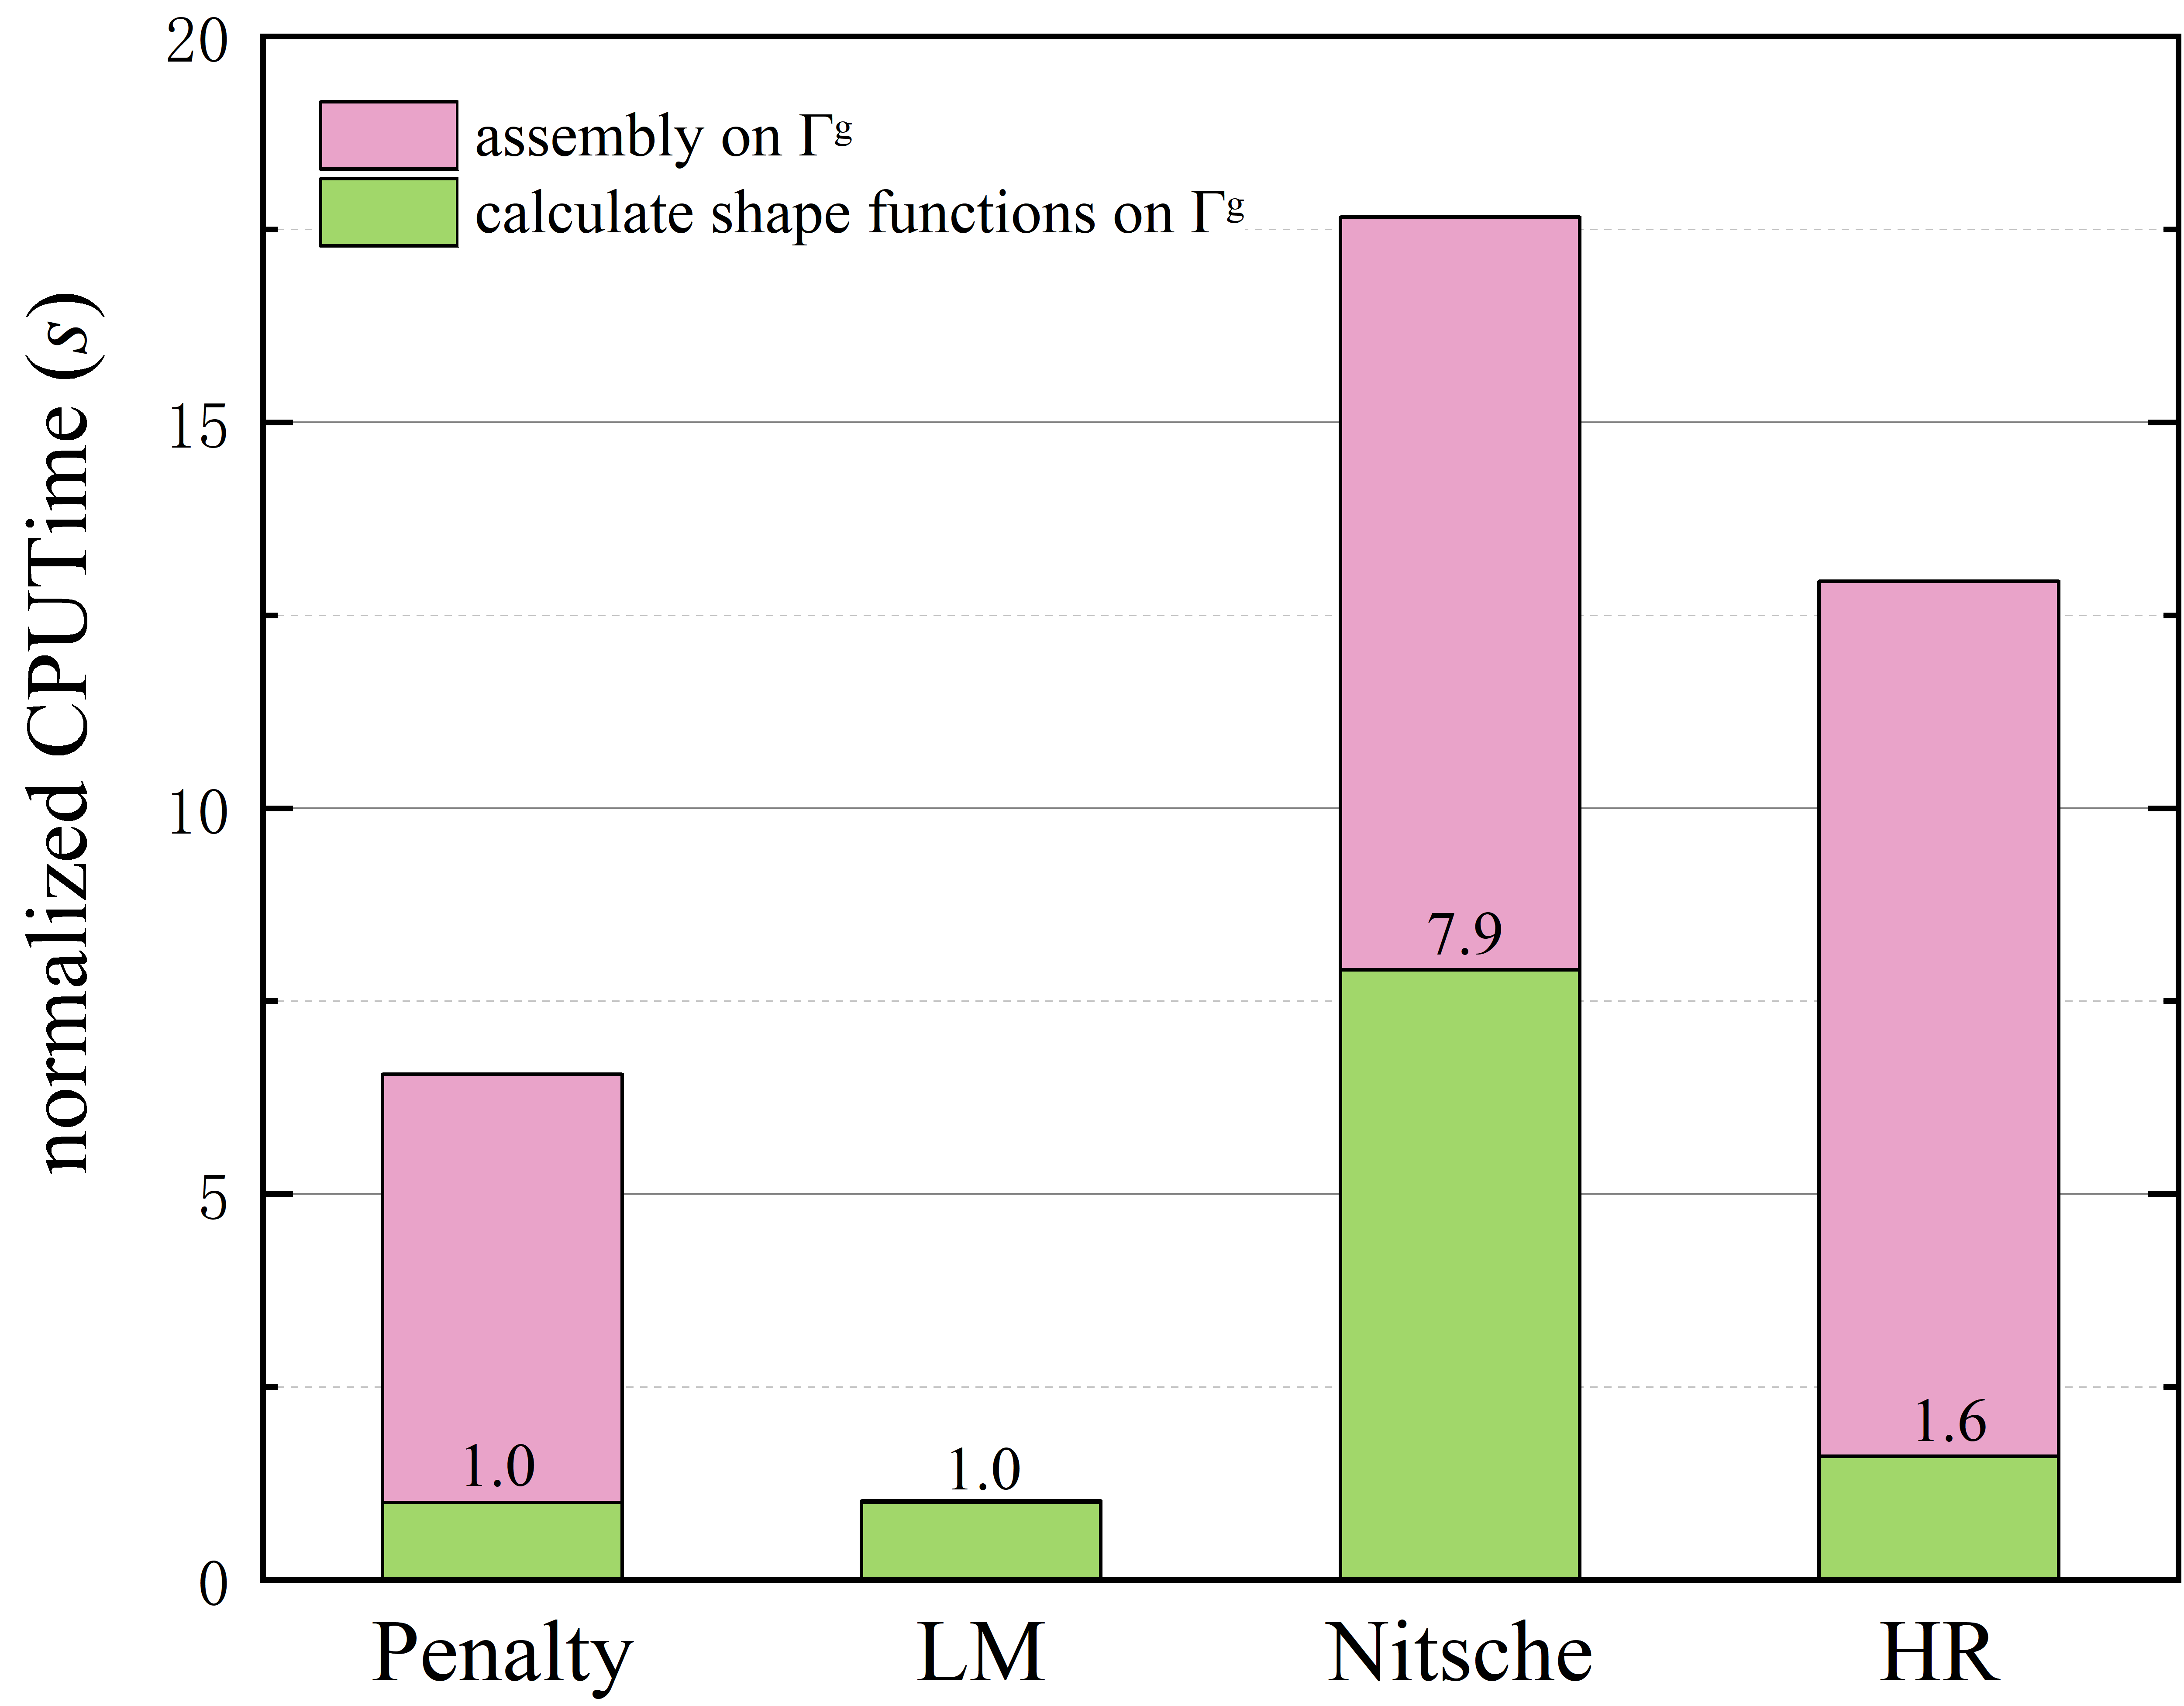
\includegraphics[scale=0.5]{figure/E/hole/caculate.png}
    \caption{带孔无限大平板问题本质边界条件施加效率分析}\label{Hcaculate}
\end{figure}
% 最后,图(\ref{Hstress})为带孔无限大平板问题的应力云图,从图中可以看出RKGSI-Penalty法和精确解之间是有差异的,
% 而RKGSI-Nitsche法和RKGSI-HR法是和精确解几乎相同。但Nitsche法是需要依靠人工经验参数并且计算效率也低于HR法。
\begin{figure}[H]
    \centering
    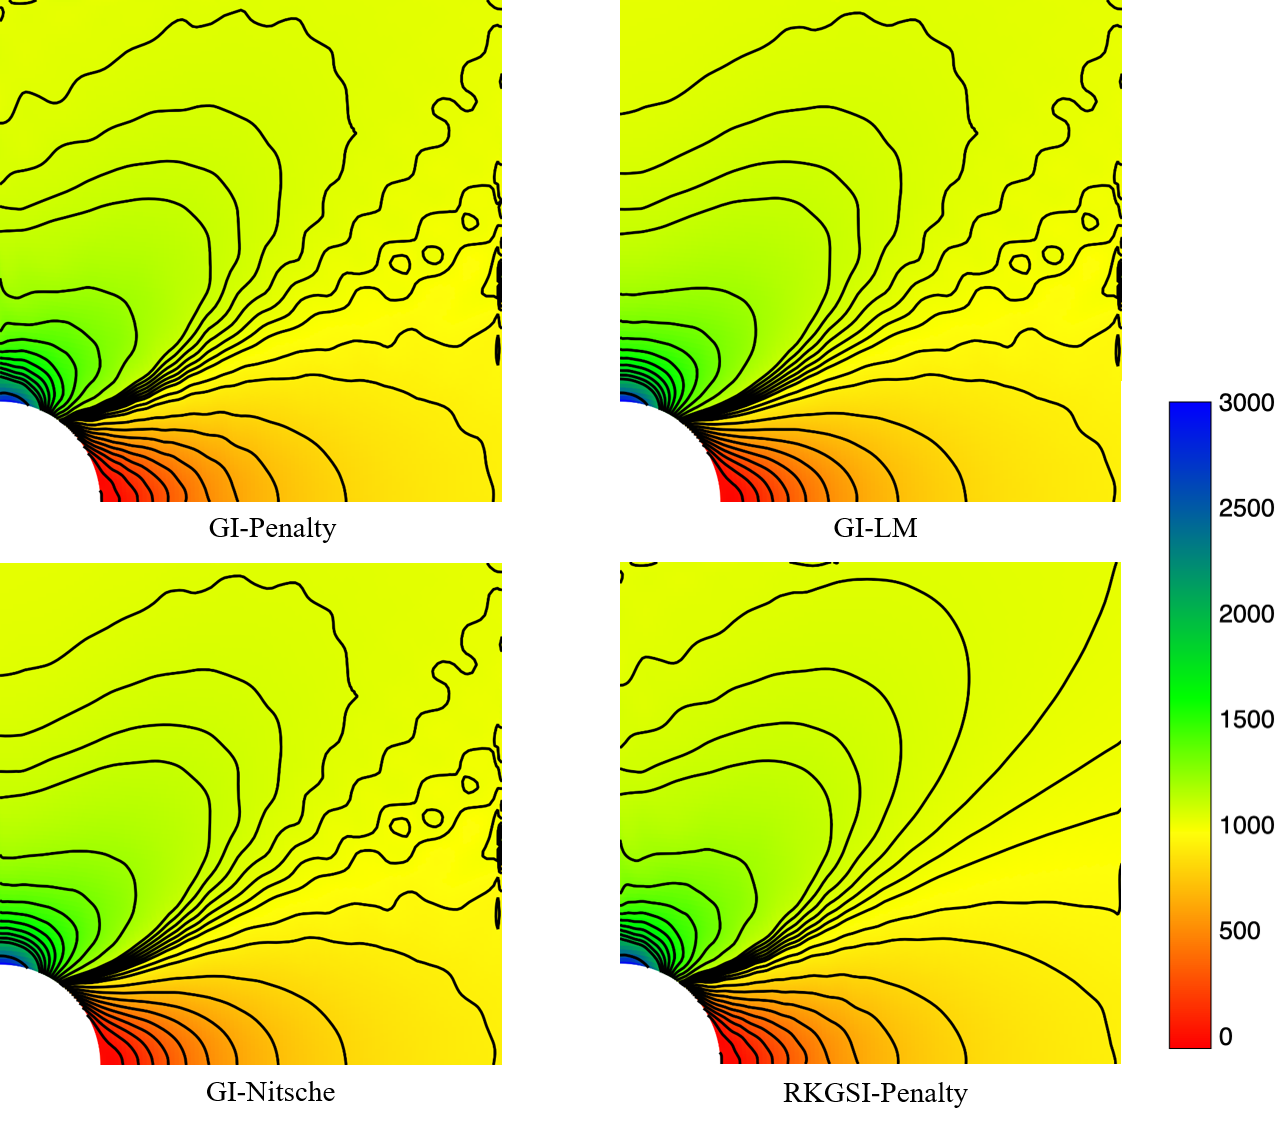
\includegraphics[scale=0.5]{figure/E/hole/hole.stress1.png}
    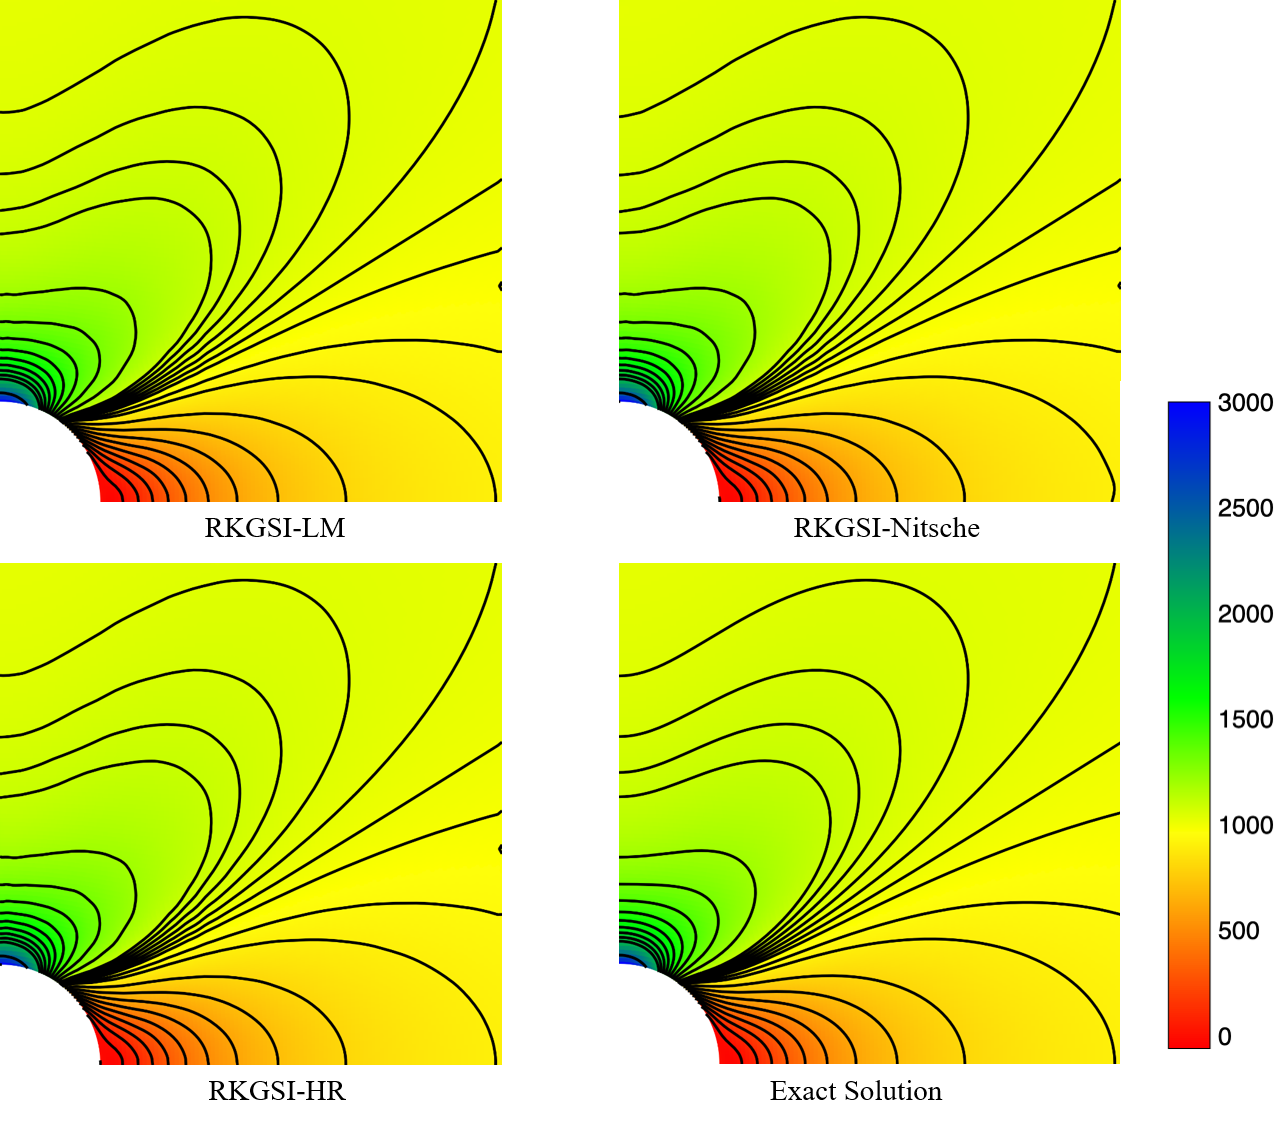
\includegraphics[scale=0.5]{figure/E/hole/hole.stress2.png}
    \caption{带孔无限大平板问题应力云图}\label{Hstress}
\end{figure}\newpage

  

